% !TeX spellcheck = de_CH
%%%%%%%%%%%%%%%%%%%%%%%%%%%%%%%%%%%%%%%%%%%%%%%%%%%%%%%%%%%%%%%%%
%  _____   ____  _____                                          %
% |_   _| /  __||  __ \    Institute of Computitional Physics   %
%   | |  |  /   | |__) |   Zuercher Hochschule Winterthur       %
%   | |  | (    |  ___/    (University of Applied Sciences)     %
%  _| |_ |  \__ | |        8401 Winterthur, Switzerland         %
% |_____| \____||_|                                             %
%%%%%%%%%%%%%%%%%%%%%%%%%%%%%%%%%%%%%%%%%%%%%%%%%%%%%%%%%%%%%%%%%
%
% Project     : BA Welti Keller
% Title       : 
% File        : software.tex Rev. 00
% Date        : 15.09.2014
% Author      : Tobias Welti
%
%%%%%%%%%%%%%%%%%%%%%%%%%%%%%%%%%%%%%%%%%%%%%%%%%%%%%%%%%%%%%%%%%

\chapter{Software}\label{chap.software}
\todo{software}

\section{Software-Stack}\label{sec.sw_stack}


\subsection{Überblick}\label{subsec.sw_ueberblick}
Die Hauptkomponenten (Abbildung \ref{fig.swlogger}) des \gls{logger}s sind die Datenablage und das Busprotokoll, welche jeweils in einem eigenen \glspl{thread} implementiert wurden, damit sie unabhängig voneinander arbeiten können. Damit die Kommunikation zwischen den Teilnehmern reibungslos funktioniert wurde eine Busverwaltung implementiert, die mehrere Aufgaben wahrnimmt. Zum einen kümmert sie sich um die Teilnehmerverwaltung und verteilt eindeutige CAN-IDs, die aus einer Konfigurationsdatei gelesen werden. Weiter weist die Busverwaltung jeweils einem Teilnehmer ein Token zu als Erlaubnis, Daten zu schicken. Damit wird sichergestellt, dass kein Sensor verhungert, weil seine Nachrichten jeweils von anderen Sensoren überschrieben werden. 

\begin{figure}
	\centering
		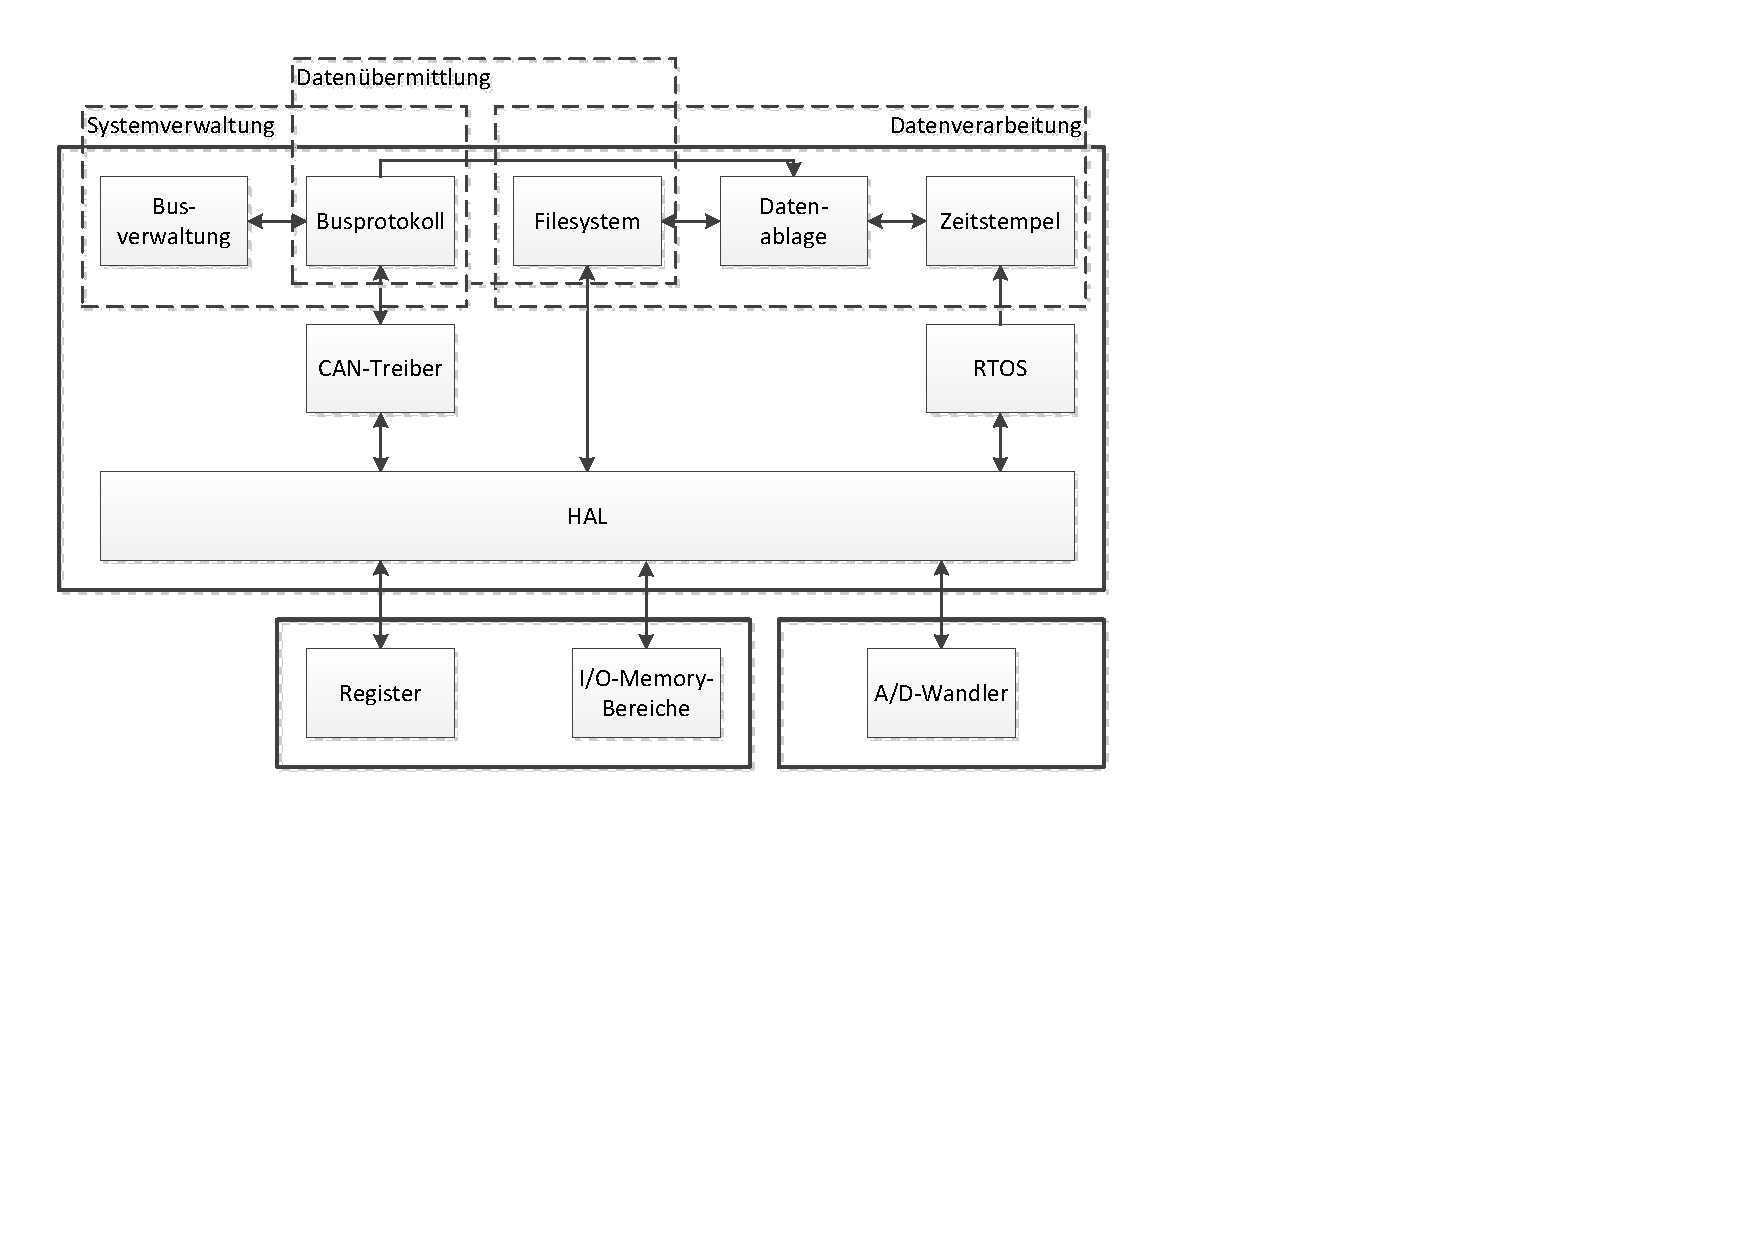
\includegraphics[width=0.8\textwidth]{images/visio/Softwarestack_Logger.pdf}
	\caption{Softwarestack des \gls{logger}s.}
	\label{fig.swlogger}
\end{figure}

Das Busprotokoll kümmert sich um die technische Kommunikation mit den \glspl{sensoreinh} am Bus und bietet Schnittstellen an, um Nachrichten abzuschicken oder eingetroffene Meldungen abzuholen. Trifft eine Meldung von einem Sensor ein wird ein Interrupt ausgelöst, der die Meldung ausliest und in einem Ringbuffer ablegt. Dieser Buffer wird periodisch vom Kommunikationsthread ausgelesen und die darauf enthaltenen Meldungen in ein Format gebracht, das für die Anwendung lesbar ist. Im Anschluss wird diese Meldung mittels einer Queue und unter Verwendung eines Memory-Pools dem Datenablage-Thread zur Verfügung gestellt. Dieser holt sich die vorbereitete Meldung und, sofern es sich dabei um Messdaten handelt, schreibt diese in die Datendatei der sendenden \gls{sensoreinh}. Nach der Verarbeitung der Message gibt der Datenablage-Thread den Platz im Memory-Pool wieder frei. Bei ausgehenden Nachrichten wird gleich verfahren, auch hier schreibt der Absender die Meldung in eine Queue, die dann vom Busprotokoll-Thread abgearbeitet wird. Beim \gls{logger} wurde die Queue für die eingehenden Meldungen gross genug gewählt, um ca. 800 Meldungen zwischen zu speichern, falls viele Ereignisse erfasst und übermittelt wurden. Dem gegenüber wurde die Queue für die ausgehenden Meldungen klein gehalten, da der \gls{logger} nur Steuerkommandos oder Konfigurationen an die Sensoren übermittelt, was nicht so häufig vorkommt, bzw. schnell erledigt ist.

\begin{figure}
	\centering
		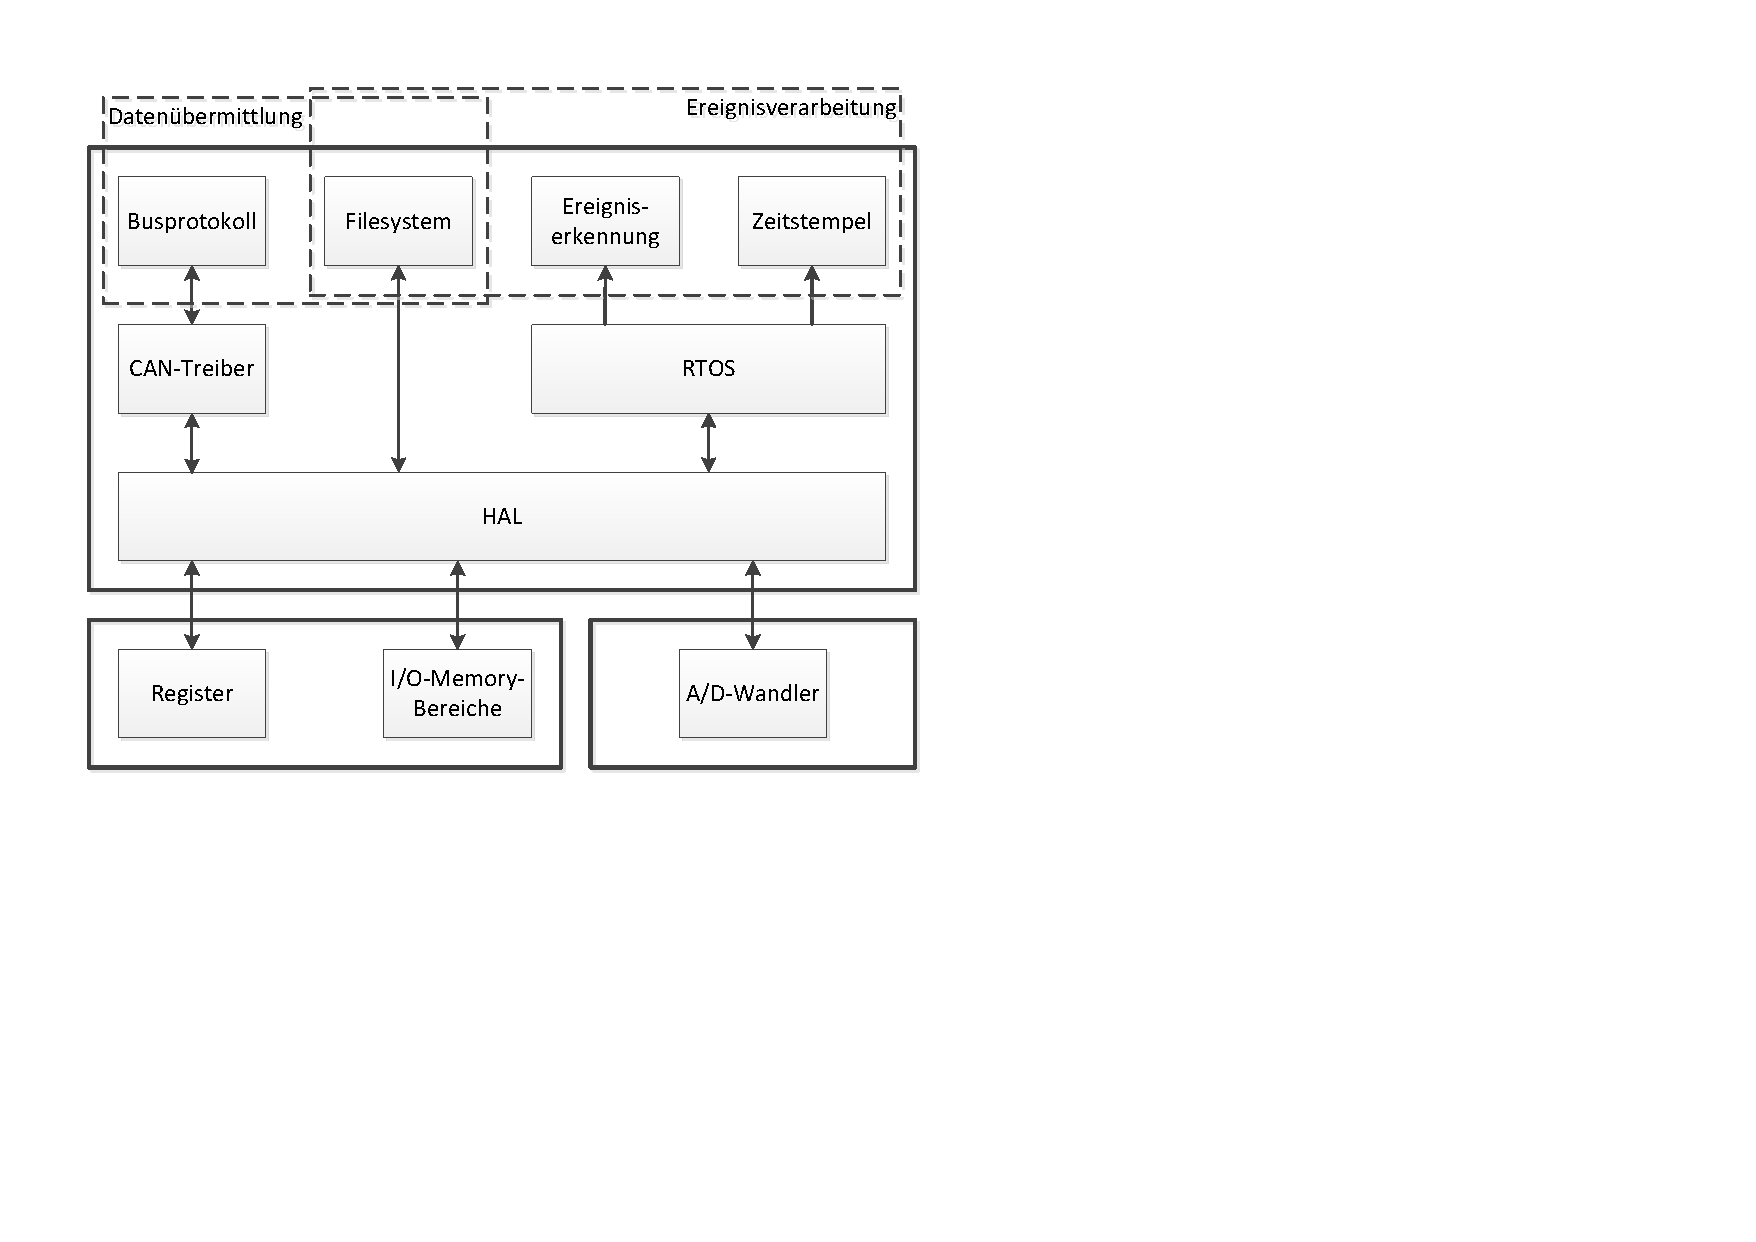
\includegraphics[width=0.8\textwidth]{images/visio/Softwarestack_Sensor.pdf}
	\caption{Softwarestack der \gls{sensoreinh}.}
	\label{fig.swsensor}
\end{figure}

Die Software der \gls{sensoreinh} (Abbildung \ref{fig.swsensor}) ist ähnlich der \gls{logger}-Software strukturiert, auch in der \gls{sensoreinh} operieren zwei Threads (Abbildung \ref{fig.commsensor}). Zum einen ist hier auch wieder der Busprotokoll-Thread anzutreffen, der wie beim \gls{logger} die ganze Kommunikation kapselt. Im zweiten Thread läuft auf der \gls{sensoreinh} die \gls{ereignisdet}, welche die Daten des angeschlossenen Beschleunigungssensors ausliest und die Ergebnisse basierend auf dem festgelegten Detail-Level aufbereitet. Ist ein Ereignis abgeschlossen (d.h. der Ausschlag des Beschleunigungssensors liegt unter einem festgelegten Schwellwert) wird dieses in die Queue zum Busprotokoll geschrieben. Hat der Sensor das Token bereits erhalten, wird er die Meldung unverzüglich übermitteln, andernfalls wird er die Message in der Queue belassen, bis ihm das Token zugewiesen wird. Damit die Queue nicht so schnell überläuft, wurde sie entsprechend gross gewählt und dient somit als eine Art Buffer. Die Queue für eingehende Meldungen bietet dafür nur wenigen Meldungen Platz, da die Sensoren einerseits nur Meldungen erhalten, die entweder an sie selbst oder als Broadcast adressiert wurden (andere Meldungen werden vom Acceptance-Filter ausgeschlossen) und andererseits nur Steuerkommandos vom \gls{logger} zu erwarten sind.

Die Abbildung \ref{fig.ipccomm} zeigt das Zusammenspiel der internen (\gls{ipc}) und externen (CAN-Bus) Kommunikation. Im \gls{logger} arbeiten drei Threads zusammen, um die Benutzereingaben (Console-Thread), die Datenverarbeitung (Processing-Thread) und die Kommunikation über den CAN-Bus abzuwickeln. In der \gls{sensoreinh} kommunizieren die \gls{ereignisdet} und der Kommunikations-Thread (CAN-Bus) miteinander.

\begin{figure}
	\centering
		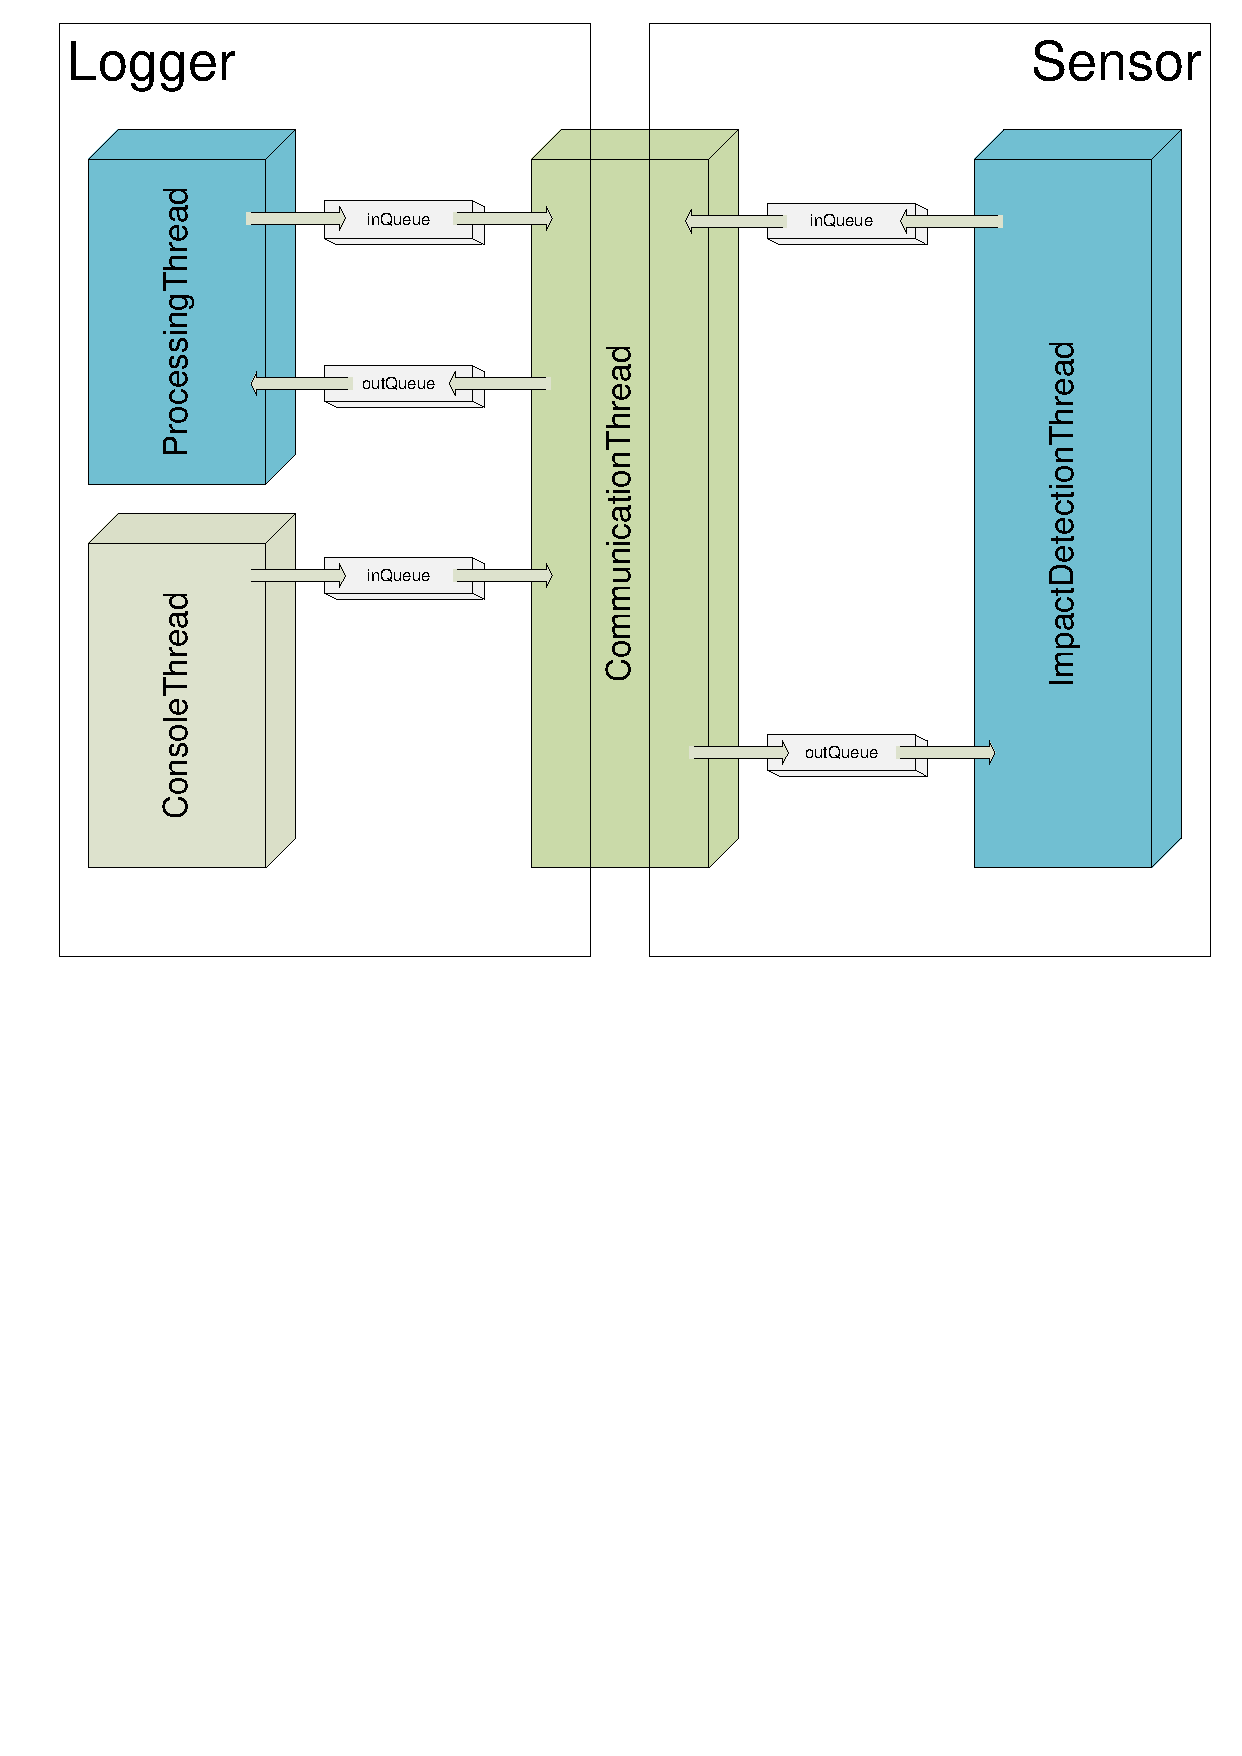
\includegraphics[width=0.8\textwidth]{images/visio/IPC-Grob.pdf}
	\caption{Interne und externe Kommunikation.}
	\label{fig.ipccomm}
\end{figure}


\subsection{Messdatenerfassung}\label{subsec.sw_messen}
Der NXP LPC4088 Mikroprozessor verfügt über einen 12-bit \gls{adwandler}, der über einen Multiplexer auf acht \glspl{pin} messen kann. Auf dem verwendeten Quickstart-Board stehen sechs \glspl{pin} für A/D-Wandlung zur Verfügung. Für die geplante Anwendung reicht ein A/D-Pin, da der Beschleunigungs-\gls{sensor} die Beschleunigung nur auf einer Achse misst. Der \gls{adwandler} des NXP LPC4088 wird mit einer \gls{fs} von 10~kHz betrieben. Falls höhere \glspl{fs} nötig sind, kann der \gls{adwandler} theoretisch mit bis zu 400~kHz betrieben werden.

\paragraph{Abtastrate} Um die \gls{fs} genau einzuhalten wird ein Ticker (Timer) des \emph{NXP LPC4088} \gls{mc}s eingesetzt, der die Messung des \gls{adwandler}s anstösst (Listing \ref{list.tickerADC}). Das Intervall des Tickers kann dynamisch konfiguriert werden. Diese Methode ist genauer als das Heruntertakten des \gls{adwandler}s, was nur in relativ groben Stufen erfolgen kann. Der Ticker löst einen Interrupt aus, der den \gls{adwandler} anstösst. Die A/D-Wandlung nimmt immer genau 31 Taktzyklen in Anspruch. Nach abgeschlossener Messung schreibt der \gls{adwandler} den Messwert in ein eigenes Register und setzt einen \gls{irq}. Der \gls{irq} signalisiert dem \gls{mc}, dass ein Messwert zur Abholung bereit liegt. Damit der Messwert so rasch wie möglich, auf jeden Fall aber vor Ablauf der nächsten Messperiode, für die weitere Verarbeitung abgeholt werden kann, hat der \gls{irq} die höchst mögliche Priorität. Der Interrupt des \gls{adwandler}s unterbricht also jeden laufenden Prozess. Das Zusammenspiel von Ticker,  \gls{adwandler}, Ereigniserkennung und Busprotokoll ist in einem Kommunikationsdiagramm in Abbildung \ref{fig.commsensor} dargestellt.

\begin{figure}
	\centering
		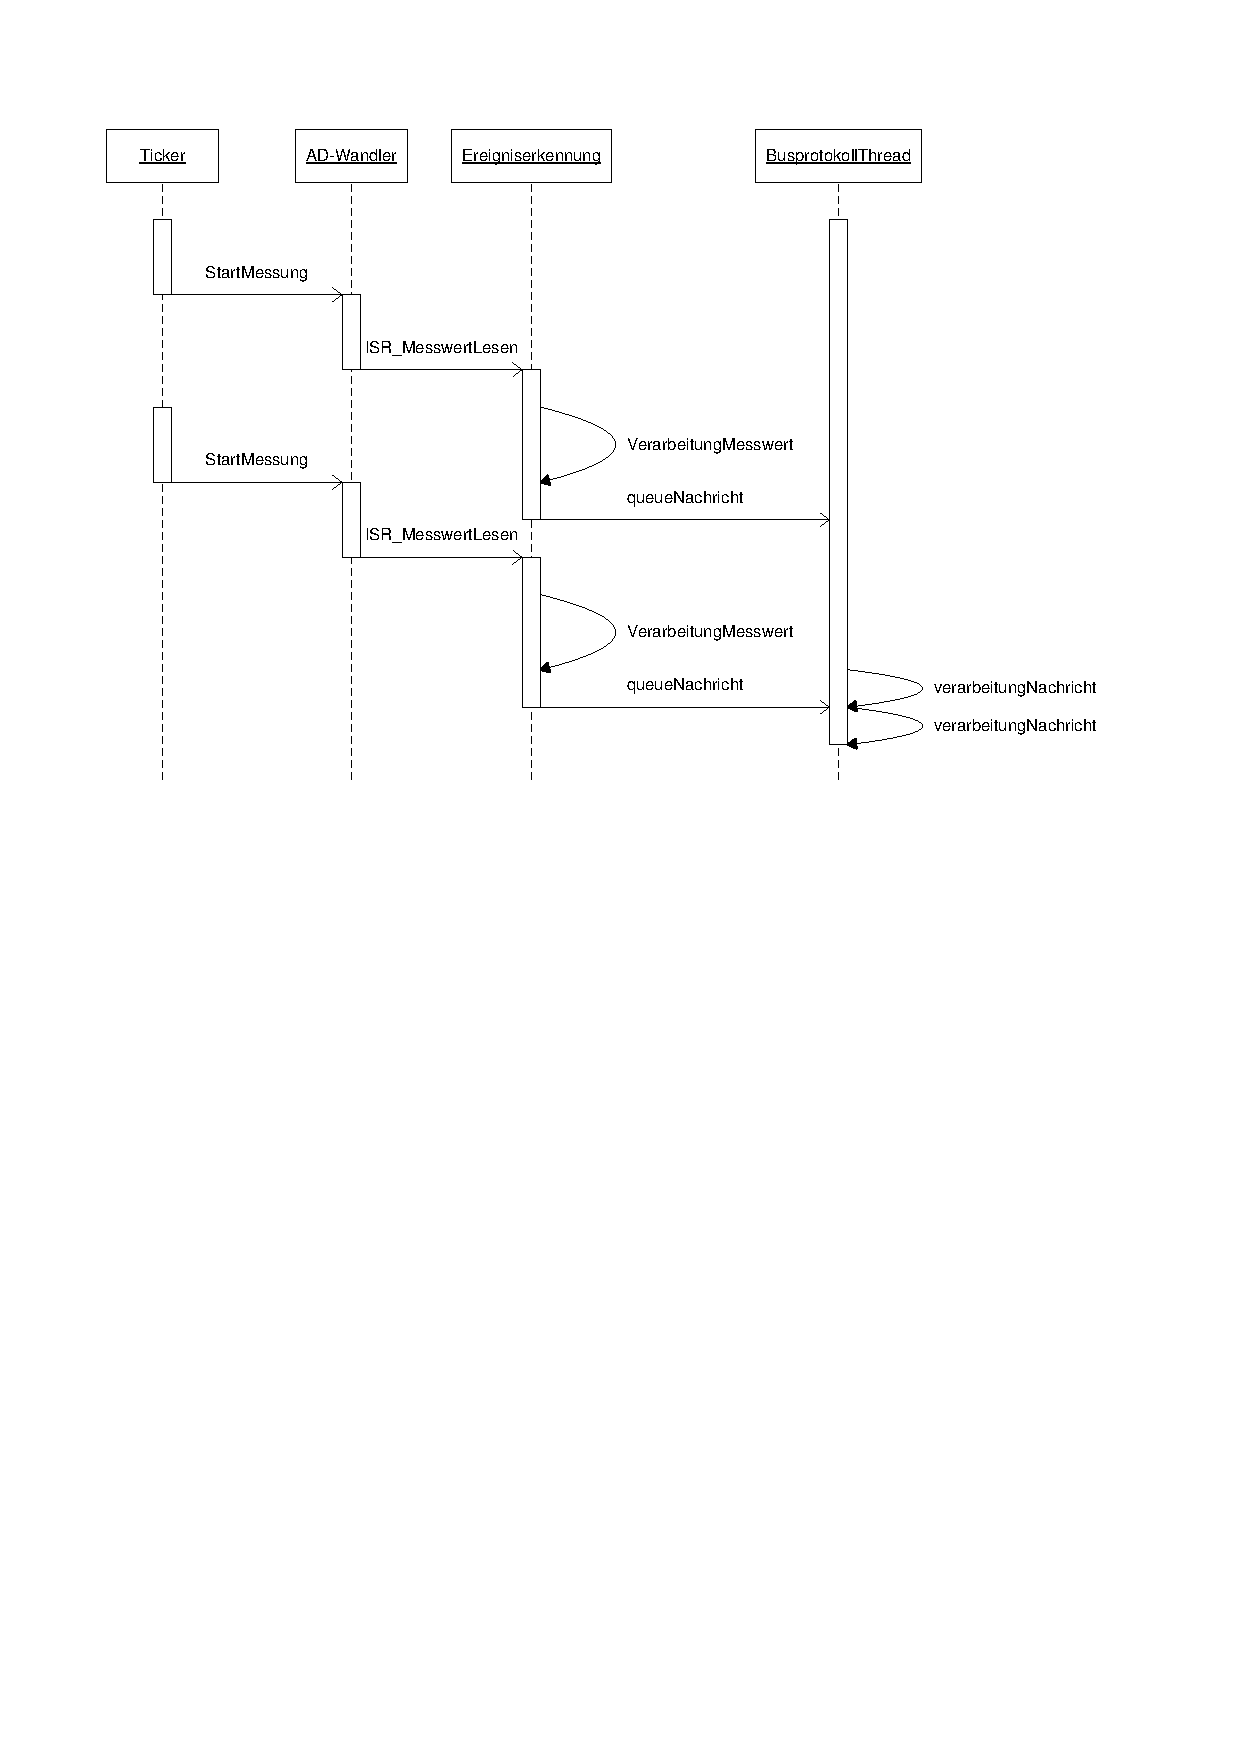
\includegraphics[width=0.8\textwidth]{images/visio/AD-Er-Com.pdf}
	\caption{Kommunikationsdiagramm der Threads in der \gls{sensoreinh}.}
	\label{fig.commsensor}
\end{figure}


\begin{lstlisting}[language=C,caption=Timer mit Aufruf der A/D-Wandler-Funktion (ADC\_4088.cpp), label=list.tickerADC]
// ISR 
void start_ADC_Conversion(){
		// start conversion when the ticker fires
		LPC_ADC->CR |=(1 << 24);
}

// ...
// register Interrupt Handler and attach ticker
int register_ADC_interrupt(analogin_s *obj, PinName pin, uint32_t ADC_IRQHandler, uint32_t interval){
  // ...
  ticker.attach_us(&start_ADC_Conversion, interval);
  // ...
}
\end{lstlisting}

\paragraph{ISR} Der \gls{mc} ruft die \gls{isr} (Listing \ref{list.isrADC}) auf, um den \gls{irq} abzuhandeln. Die \gls{isr} holt den Messwert aus dem Register und speichert ihn zusammen mit dem \gls{timestamp} in einer \gls{fifo} ab. Die \gls{isr} erhöht den \gls{timestamp} um eins für den nächsten Messwert und gibt dann die Kontrolle an den unterbrochenen Prozess zurück.

\begin{lstlisting}[language=C,caption=ISR zur Abhandlung des ADC-Interrupt Requests (impact\_event.cpp), label=list.isrADC]
void isr_nextMeasurement(){
	// read ADC measurement from Register, automatically resets IRQ
	value = LPC_ADC->GDR;
	value = (value >> 4) & 0xFFF;
	timestamp++;
	
	enqueue_impact_input(timestamp, value);
}
\end{lstlisting}

Sobald das Ereignis abgeschlossen ist (siehe \ref{subsec.sw_ereignis}), wird es mittels einer Queue asynchron dem Kommunikationsthread zur Verfügung gestellt, der die Meldungen dem Logger weiterleitet, sofern der Bus frei ist und der aktuelle Sensor den Token zur Datenübermittlung erhalten hat.

\paragraph{Timestamp} Der Timestamp muss zwingend in der \gls{isr} (Listing \ref{list.isrADC}) erhöht werden, damit er immer sofort nach der Erfassung eines neuen Messwerts aktualisiert wird. Würde der Timestamp mittels einem zweiten Timer und einer zweiten \gls{isr} erhöht, bestünde die Gefahr einer ungeregelten Reihenfolge der Abarbeitung der \gls{irq}s. Mal würde der \gls{timestamp} vor dem Kopieren der Messdaten erhöht, mal erst danach.

\paragraph{Datenauswertung} Die Datenauswertung wird in regelmässigen Abständen aufgerufen und arbeitet die \gls{fifo} mit den neuen Messwerten ab, um Ereignisse zu erkennen. Der Aufruf der \gls{ereignisdet} ist nicht so stark an einen genauen Takt gebunden wie die A/D-Wandlung, da die \gls{fifo} genügend gross ist, um mehrere hundert Messwerte zwischenzuspeichern. Ein Thread ruft die \gls{ereignisdet} auf und wartet nach Beendigung der Subroutine 1~ms.

\subsection{Ereigniserkennung}\label{subsec.sw_ereignis}
\subsubsection{Hilbert-Transformation}
Von der \gls{wsl} wurde die \gls{ereignisdet} bisher mittels \gls{hilbert} gelöst. Die \gls{hilbert} liefert die umhüllende Kurve des gemessenen \gls{signal}s. Überschreitet die Umhüllende den \gls{threshold}, markiert dies den Start eines neuen \gls{ereignis}ses. Fällt die Umhüllende unter den \gls{threshold}, ist das \gls{ereignis} beendet. Abbildung \ref{fig.wslcurve} zeigt ein Beispiel von Messdaten aus einer bestehenden Anlage. Die Hüllkurve wurde von Hand eingezeichnet, um das Verfahren zu demonstrieren. Die \glspl{ereignis} werden als 'packet' bezeichnet, die Peaks als 'Impulses'.

\begin{figure}
	\centering
		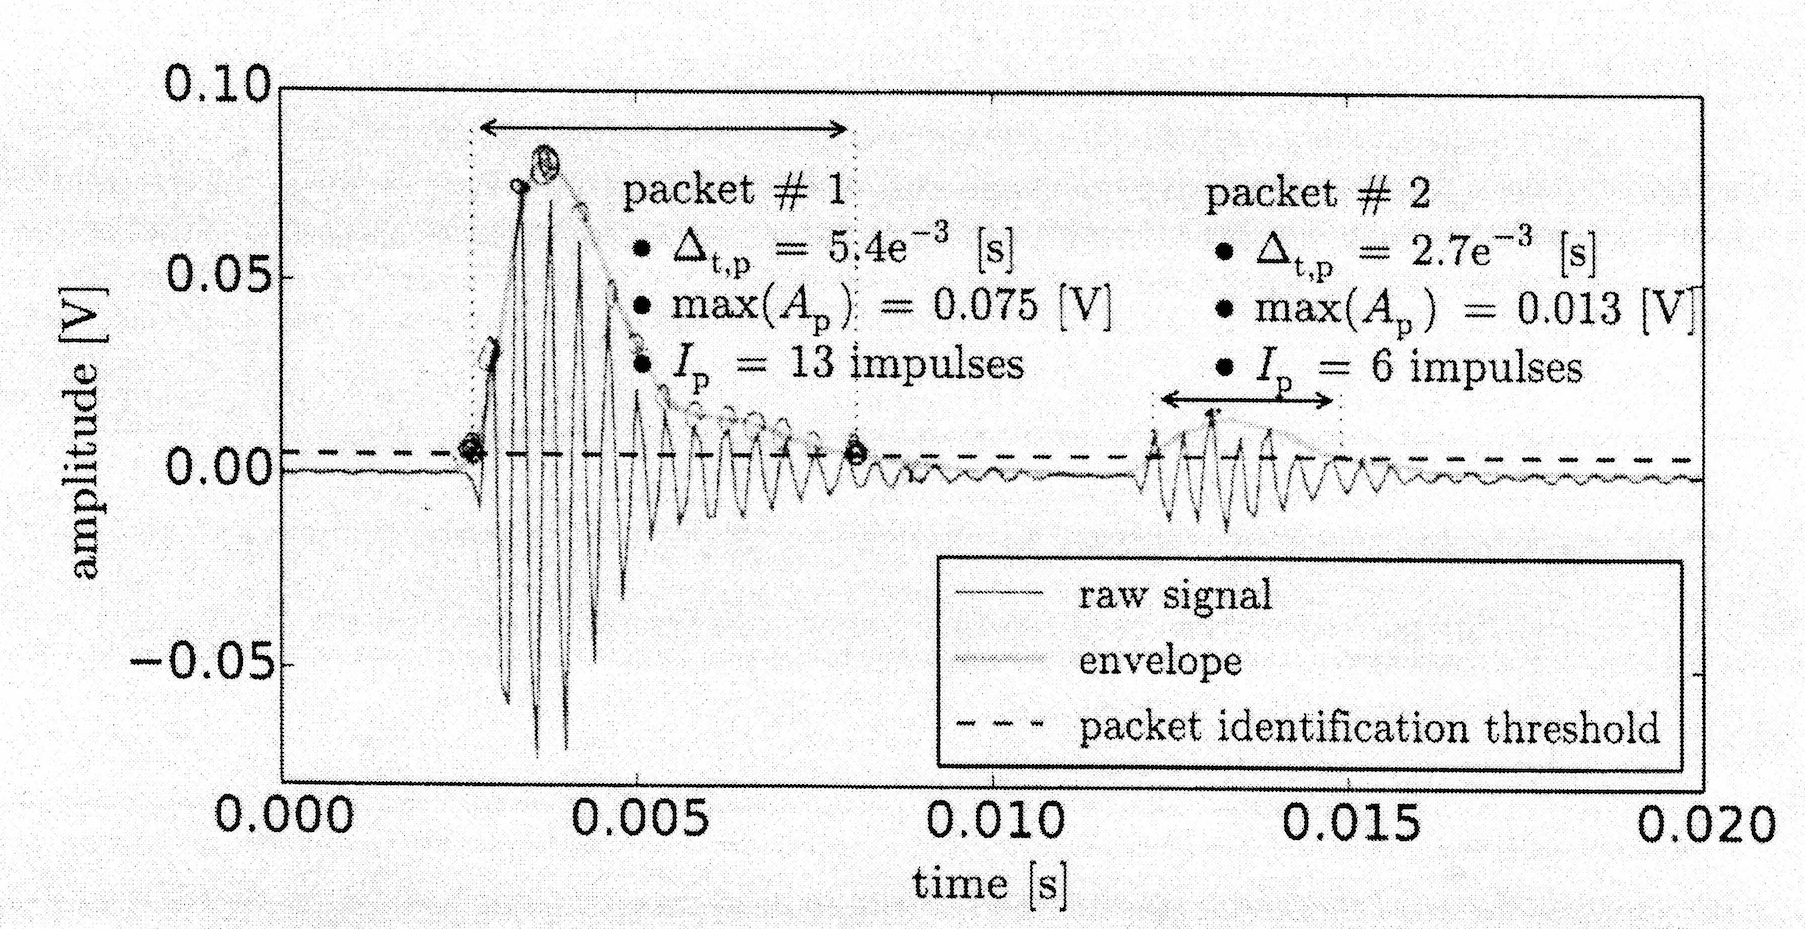
\includegraphics[width=0.8\textwidth]{images/curve_wsl.png}
	\caption{Beispiel von Messdaten mit einer Hüllkurve (envelope).}
	\label{fig.wslcurve}
\end{figure}

Die Berechnung der \gls{hilbert} erfordert einigen Aufwand. Durch \gls{dft} wird das Spektrum des Signals berechnet. Negative Frequenzanteile werden auf null gesetzt und das resultierende Spektrum mittels \gls{idft} wieder in ein Signal umgerechnet (vgl. \cite{wiki_hilbert}). Das resultierende Signal umhüllt das Eingangssignal. 

Für die \gls{dft} und die \gls{idft} ist der Rechenaufwand je \ensuremath{N \cdot log_2(N)}. Je mehr Datenpunkte in einem Schritt verrechnet werden (\gls{blockg}), desto höher ist der Aufwand, aber desto genauer ist das Resultat. Mit einer \gls{blockg} von 128 Messwerten benötigt die \gls{dft} und die \gls{idft} je 896 komplexe Multiplikationen und Additionen (vgl. \cite[Kap. 3, S. 48]{dsv1_hilbert}). Pro Messwert sind das 7 komplexe Multiplikationen und Additionen. Dank der DSP-Fähigkeiten des gewählten Cortex\texttrademark -M4 Prozessors liegt die zu erwartende Prozessorauslastung für die \gls{hilbert} bei einer \gls{fs} von \ensuremath{10~kHz} bei wenigen Prozent.

\subsubsection{Hilbert-Transformation als FIR-Filter}
Die \gls{hilbert} kann mittels eines \gls{fir}s angenähert werden. Ein Allpass mit gerader Filter-Ordnung und geeignet gewählten Koeffizienten (Abbildung \ref{fig.hilbertFIR}) liefert eine gute Näherung. Je nach gewählter Ordnung des Filters ist der Rechenaufwand aber in ähnlicher Grössenordnung wie mit \gls{dft} und \gls{idft}.
\begin{figure}
	\centering
		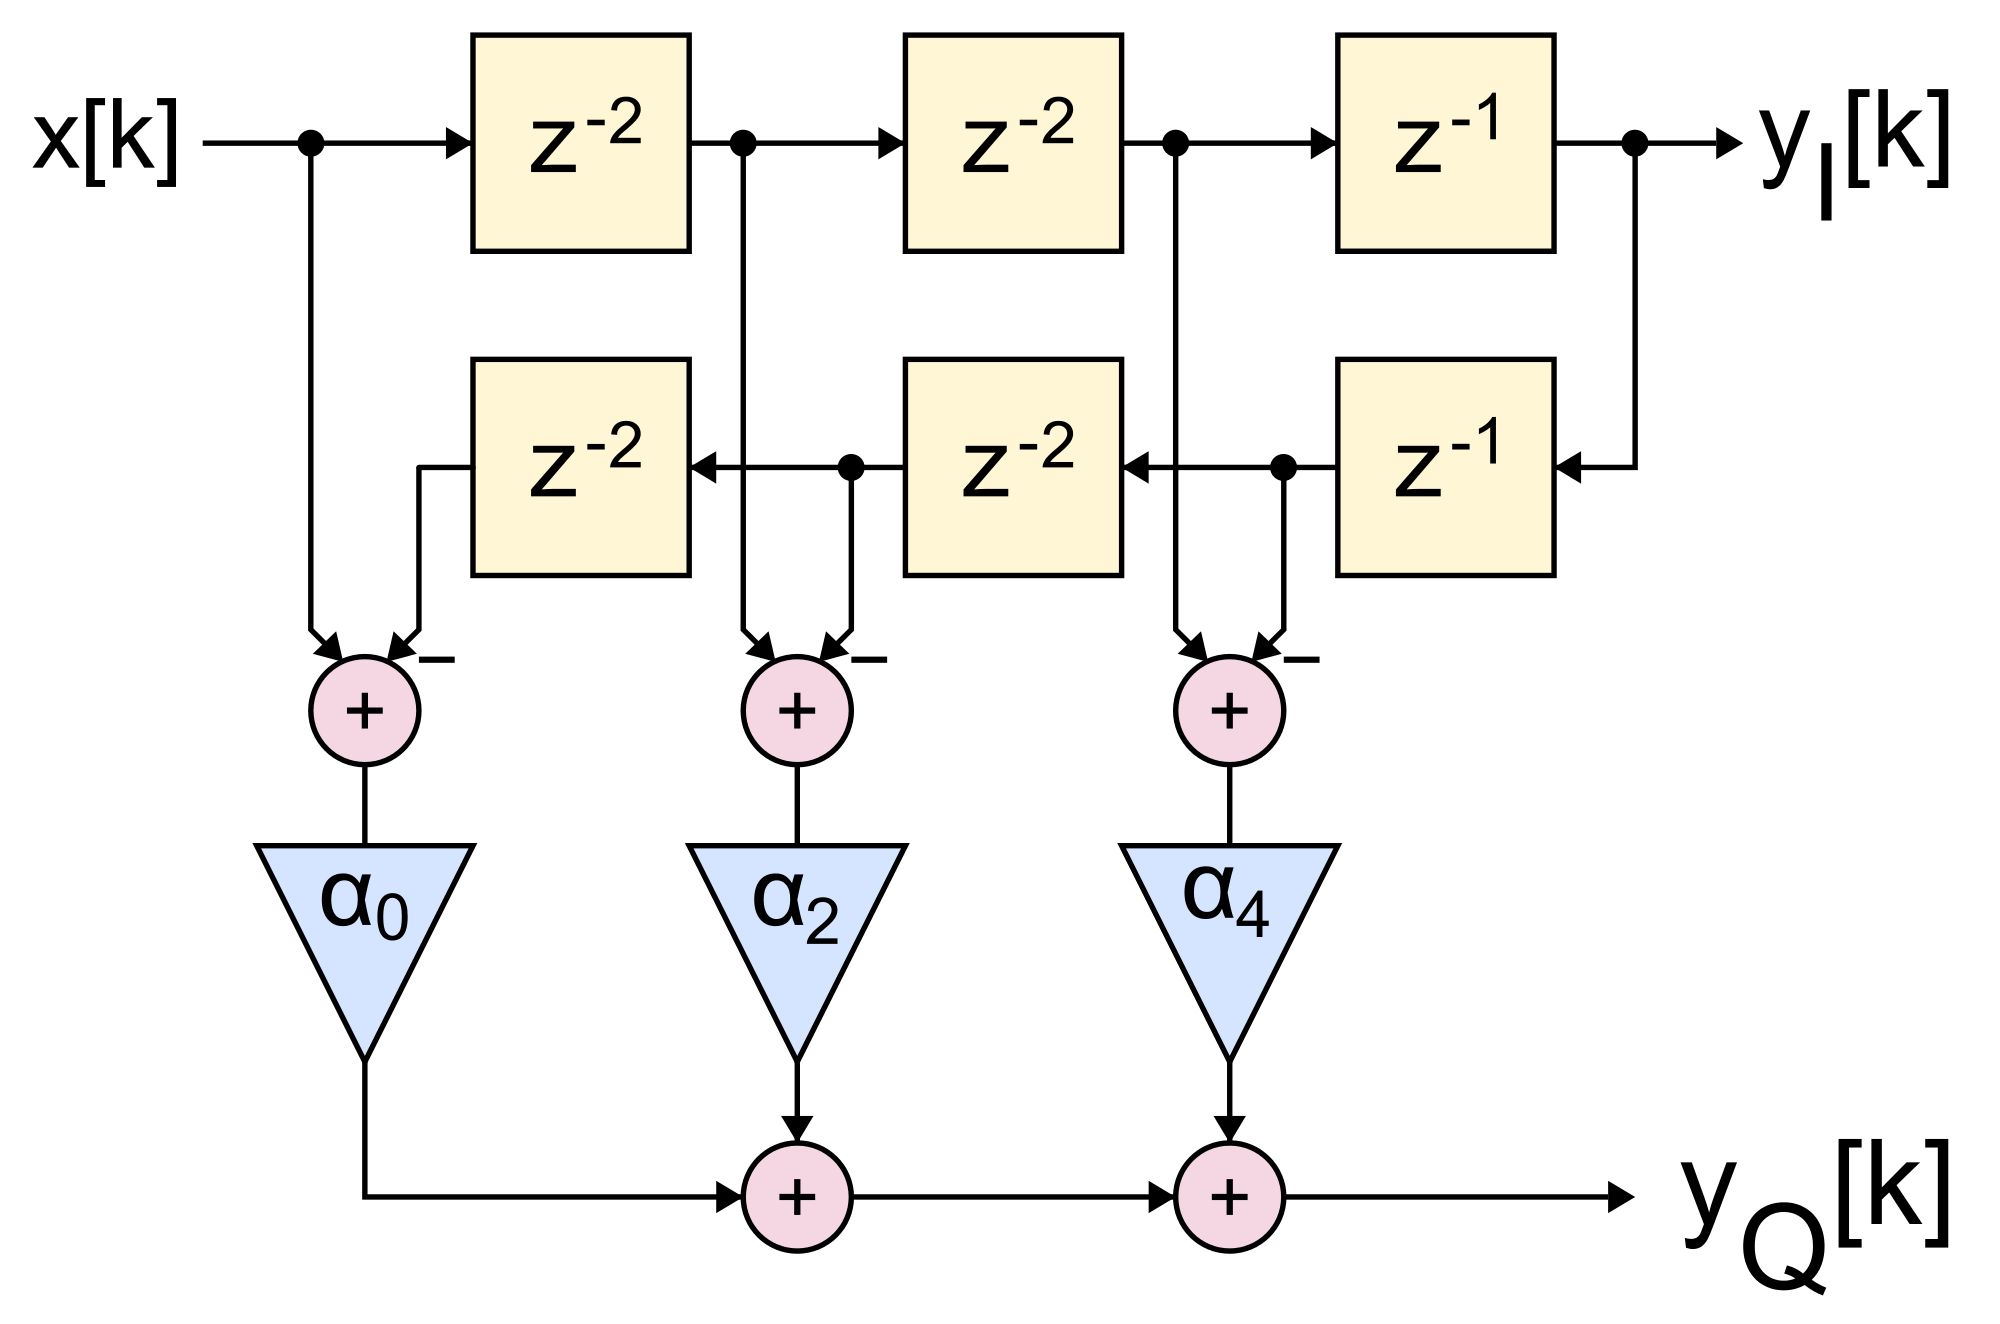
\includegraphics[width=0.8\textwidth]{images/FIR_Hilbert_Transform_Filter.png}
	\caption{\gls{hilbert} als \gls{fir} \cite{wiki_hilbertFIR}.}
	\label{fig.hilbertFIR}
\end{figure}

\subsubsection{Zustandsmaschine}
Um den Rechenaufwand der Hilbert-Transformation zu umgehen, lösen wir die \gls{ereignisdet} mittels einer \gls{fsm}. Das Zustandsdiagramm der \gls{fsmgloss} in Abbildung \ref{fig.fsm_impact_detection} zeigt alle möglichen Zustände der \gls{fsm} sowie welche Ereignisse einen Übergang in einen anderen Zustand auslösen.

\begin{figure}
	\centering
		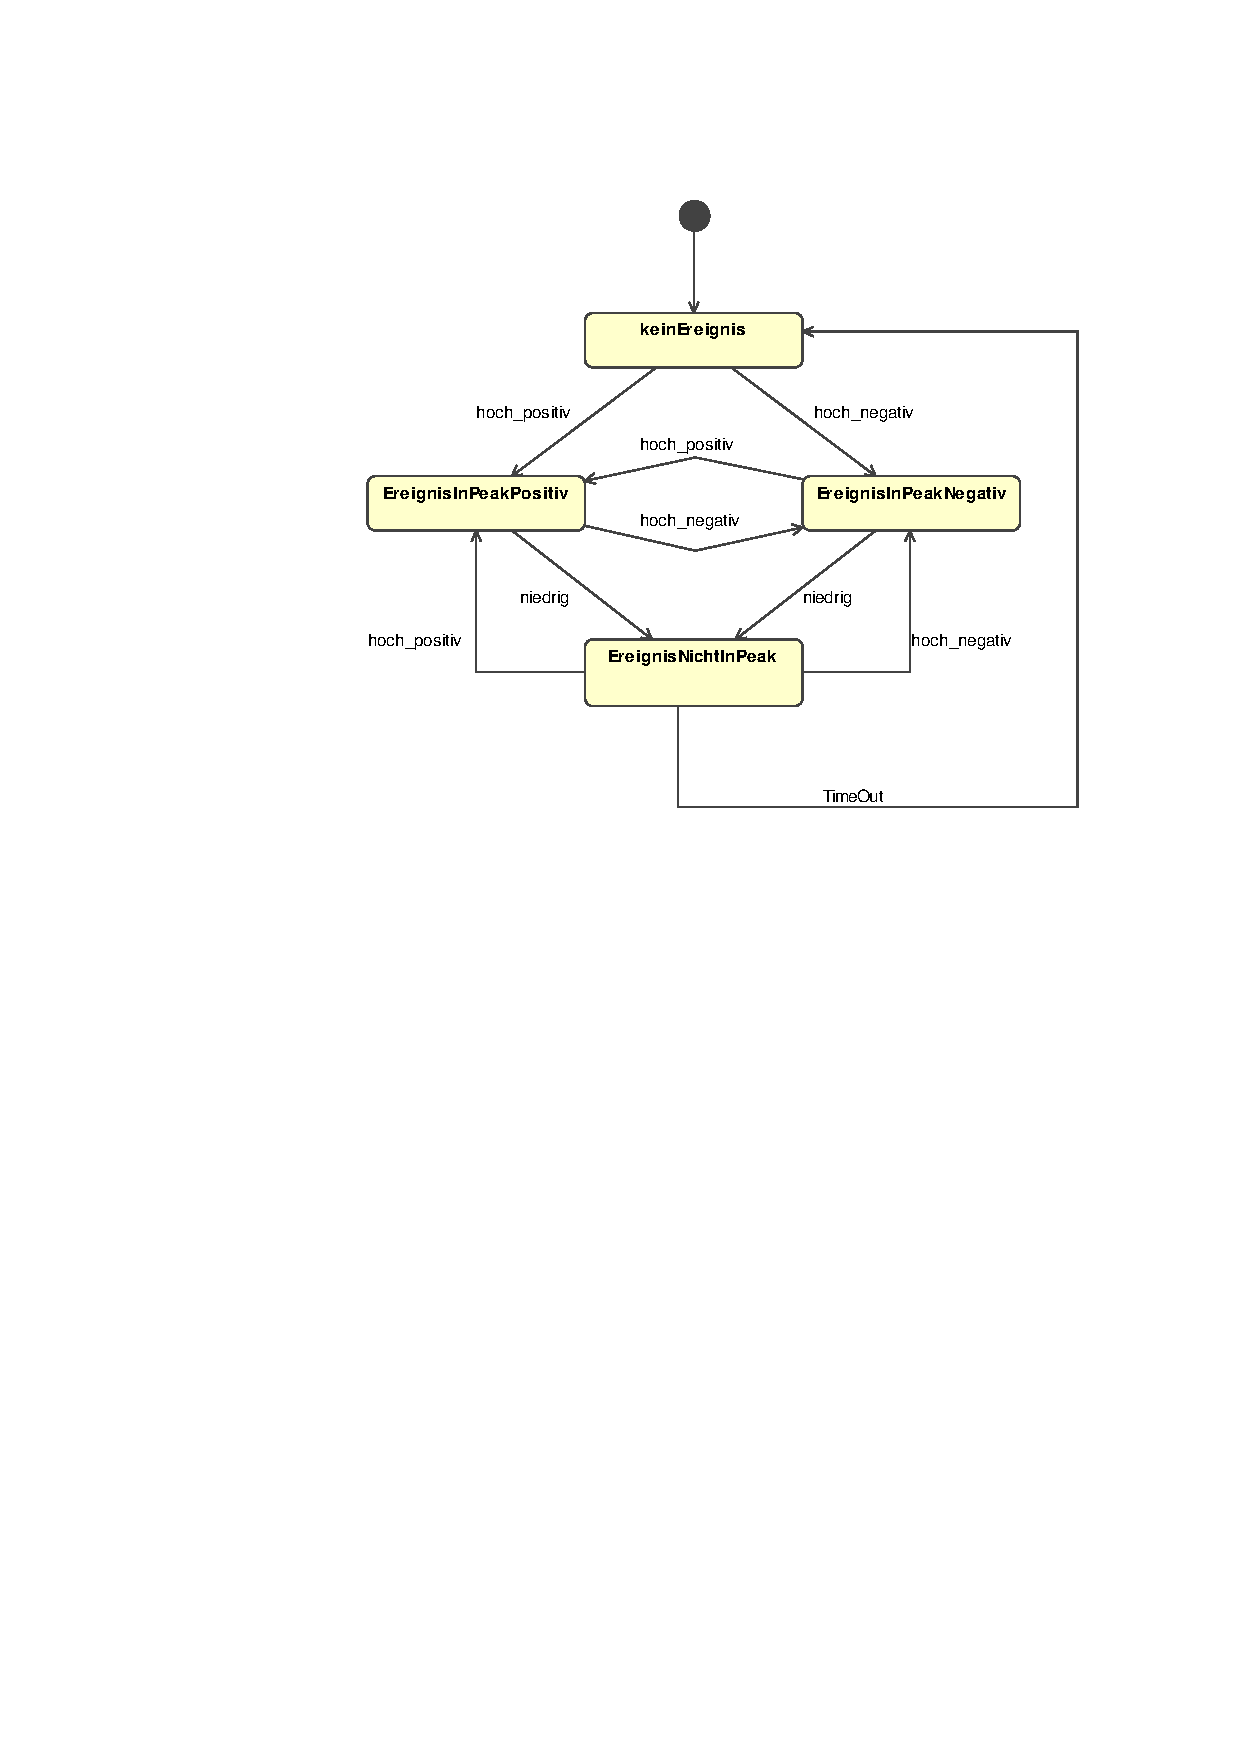
\includegraphics[width=0.8\textwidth]{images/magicdraw/Ereigniserkennung.pdf}
	\caption{Zustandsmaschine der Ereigniserkennung.}
	\label{fig.fsm_impact_detection}
\end{figure}

\paragraph{Konfiguration der Zustandsmaschine}
 Über Parameter wird definiert, welche Signalform als \gls{ereignis} erkannt werden soll. In Abbildung \ref{fig.impact_detection_params} sind die Parameter dargestellt. 
\begin{figure}
	\centering
	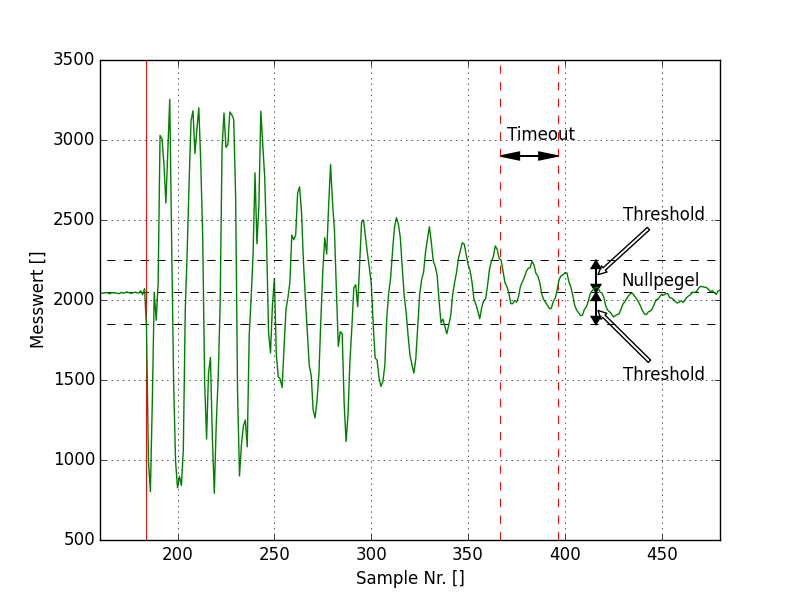
\includegraphics[width=0.8\textwidth]{images/impact_params.png}
	\caption{Parameter der Ereigniserkennung.}
	\label{fig.impact_detection_params}
\end{figure}

\paragraph{Nullpegel} Der \gls{nullpegel} kann angepasst werden, um die Erdanziehung, die als Beschleunigung auf den Sensor wirkt, zu kompensieren. Je nachdem wie der Sensor orientiert ist, ist die Erdanziehungskraft nicht parallel zur Mess-Achse des Sensors. Die vom Sensor gemessene Erdanziehungskraft in Richtung der Mess-Achse ist damit nicht immer gleich gross. Deshalb muss der \gls{nullpegel} angepasst werden können. Die mittlere gestrichelte schwarze Linie in Abbildung \ref{fig.impact_detection_params} stellt den \gls{nullpegel} dar.

\paragraph{Threshold} Der \gls{threshold} definiert, ab welcher Abweichung des Signalpegels vom Nullpegel die \gls{fsm} einen Messwert als 'hoch' betrachten soll. Zu beachten ist, dass der \gls{threshold} auf beide Seiten des Nullpegels gilt. Da der Sensor sowohl Beschleunigungen nach oben wie auch nach unten erfährt, unterscheidet die \gls{fsm} dies mit den Ereignissen 'hoch\_positiv' resp. 'hoch\_negativ'. Signalpegel, die den Threshold nicht überschreiten, werden als 'niedrig' eingestuft. In Abbildung \ref{fig.impact_detection_params} ist das erste Erreichen des (negativen) \gls{threshold}s mit einer vertikalen roten Linie markiert.

\paragraph{Timeout} Da ein Ereignis aus mehr als einem \gls{peak} besteht, muss eine Dauer (\gls{timeout}) definiert werden können, während der die \gls{fsm} auf den Beginn eines neuen \gls{peak}s wartet. Tritt während des \gls{timeout}s kein neuer Peak auf, gilt das Ereignis als beendet. Die gestrichelten roten Linien in Abbildung \ref{fig.impact_detection_params} zeigen den Timeout.

\subsubsection{Ablauf der Zustandsmaschine}
Im Folgenden wird der Ablauf in der Zustandsmaschine genauer erklärt. Im Zustandsdiagramm in Abbildung \ref{fig.fsm_impact_detection} sind die Namen der Zustände und Ereignisse ersichtlich. Der Übersichtlichkeit halber wurde auf die Auflistung der Aktionen im Diagramm verzichtet.

Die \gls{fsm} wird im Zustand 'keinEreignis' initialisiert. Tritt ein Messwert auf, der als 'hoch\_positiv' klassiert wird, wechselt die \gls{fsm} in den Zustand 'EreignisInPeakPositiv'. In diesem Zustand verbleibt die \gls{fsm}, bis ein anders klassierter Messwert eintrifft. 

Ein Messwert 'niedrig', also unterhalb des \gls{threshold}s, führt zu einem Übergang in den Zustand 'EreignisNichtInPeak'. Dieser Übergang startet einen Timer, der während der im Parameter 'Timeout' definierten Anzahl Messwerte läuft. Falls die \gls{fsm} bis zum Ablauf des Timers keinen Messwert 'hoch\_positiv' oder 'hoch\_negativ' erhält, wechselt sie wieder in den Zustand 'keinEreignis' und übergibt die Ereignisdaten dem Prozess, der für die Übertragung zum \gls{logger} zuständig ist. 

Der Timer läuft nicht in Echtzeit, sondern zählt die Anzahl Messwerte seit seinem Start, da die Verarbeitung asynchron zur Erfassung der Messwerte läuft. Das bedeutet, dass die Verarbeitung problemlos während mehreren Messwerten stillstehen kann, ohne dass Messwerte verloren gehen. Dies ist möglich, da die Messwerte in eine Warteschlange (\gls{fifo}) geschrieben werden, von wo sie von der \gls{fsm} abgeholt werden. So lange die \gls{fifo} nicht überfüllt wird, gehen keine Messwerte verloren. Die Verarbeitung der Messwerte in der \gls{fsm} erfolgt im \emph{NXP LPC4088} \gls{mc} schnell genug, um theoretisch mit einer \gls{fs} bis \ensuremath{200~kHz} messen zu können.

Falls die \gls{fifo} doch einmal überlaufen sollte, wird eine Nachricht an den \gls{logger} übertragen, der eine entsprechende Meldung in die Datendatei der \gls{sensoreinh} einträgt. Dies bedeutet, dass zu diesem Zeitpunkt einige Messwerte verloren gegangen sind. Da der \gls{timestamp} in der \gls{sensoreinh} trotzdem mit jedem \gls{sample} erhöht wird, stimmen die Zeitangaben in der Datendatei weiterhin. Es besteht lediglich eine Lücke im Datensatz.

\subsection{Detail-Level}
Je nach Einsatz der Messstation variiert die benötigte unbeaufsichtigte Messdauer von einigen Tagen bis zu mehreren Monaten. Die zu speichernde Datenmenge muss an diese Dauer angepasst werden können. Für einen langen Einsatz werden von Vorteil weniger detaillierte Messdaten abgespeichert, während für einen eher kurzen Einsatz unter Umständen sogar unkomprimierte Daten abgespeichert werden können.

Für die Wahl einer geeigneten Datenrate stehen vier verschiedene Modi, sog. Detail-Level zur Verfügung. 

Im 'raw'-Modus werden Rohdaten gespeichert (Abbildung \ref{fig.det_raw}). Dieser Modus soll hauptsächlich der Gewinnung von Kalibrierungsdaten dienen, da hier sehr viele Daten anfallen. Es wird empfohlen, nur wenige Sensoren in diesen Modus zu versetzen.

Im 'detailed'-Modus werden von jedem Ereignis alle Datenpunkte gespeichert (Abbildung \ref{fig.det_det}). Die uninteressanten Datenpunkte zwischen den Ereignissen werden nicht übertragen und aufgezeichnet. Dieser Modus ist sowohl für kurze als auch für längere Messperioden interessant, da er nur interessante Daten aufzeichnet. Die Menge anfallender Daten hängt direkt von der Häufigkeit der Ereignisse ab.

Der 'peaks only'-Modus zeichnet die Dauer des \gls{ereignis}ses sowie Zeitpunkt und Intensität aller \gls{peak}s eines \gls{ereignis}ses auf. Damit ist ein grosser Teil der Information des 'detailed'-Modus vorhanden, aber in geringerer zeitlicher Auflösung.

Der 'sparse'-Modus liefert lediglich die Dauer des \gls{ereignis}ses, die Anzahl Peaks und den maximalen Ausschlag. Dies ist eine minimale Informationsmenge, die dennoch eine Aussage über das \gls{geschiebekorn} zulässt.

Eine ausführliche Beschreibung der Detail-Level ist in der Bedienungsanleitung ab Abschnitt \ref{ssec.detaillevel}, Seite \pageref{ssec.detaillevel} zu finden.

\begin{figure}
\centering
\begin{minipage}{0.5\textwidth}
\centering
		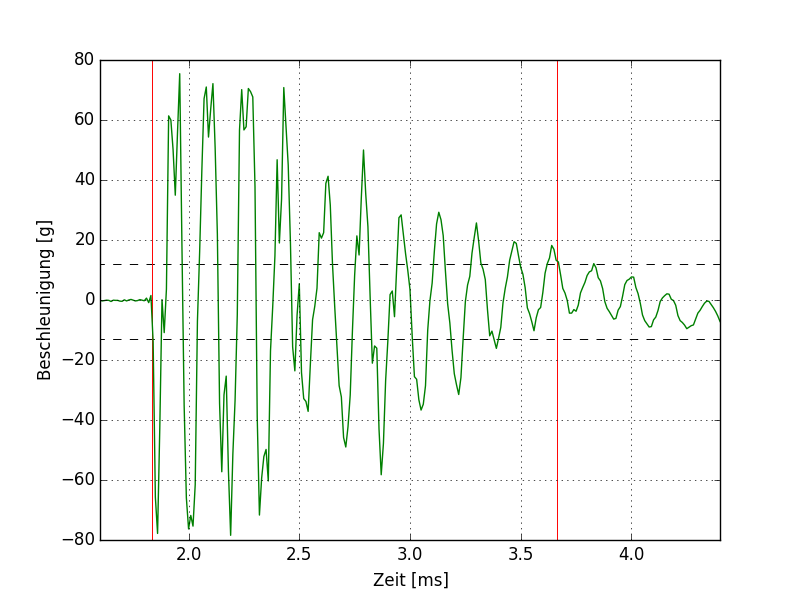
\includegraphics[width=0.95\textwidth]{images/rawshort.png}
	\captionof{figure}{Detail-Level 'raw'.}
	\label{fig.det_raw}
\end{minipage}%
\begin{minipage}{0.5\textwidth}
\centering
		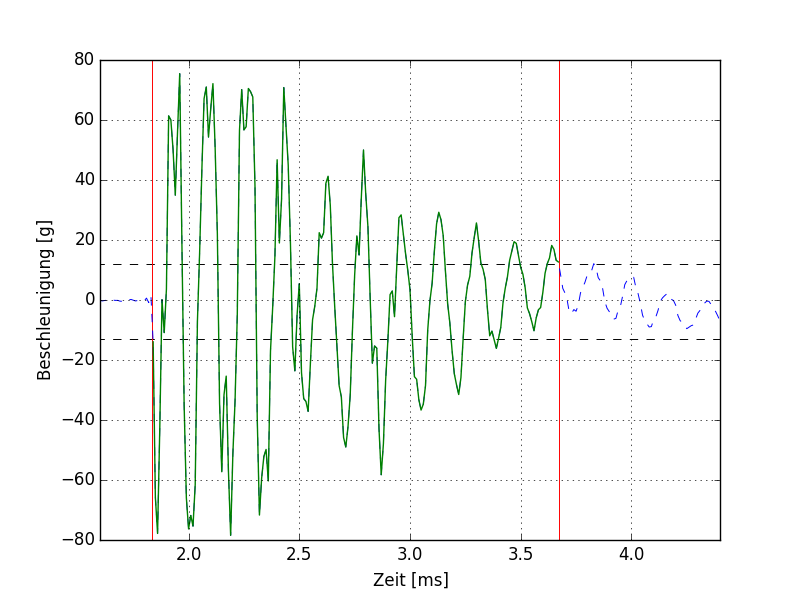
\includegraphics[width=0.95\textwidth]{images/detailed.png}
	\captionof{figure}{Detail-Level 'detailed'.}
	\label{fig.det_det}
\end{minipage}
\end{figure}

\begin{figure}
\centering
\begin{minipage}{0.5\textwidth}
\centering
		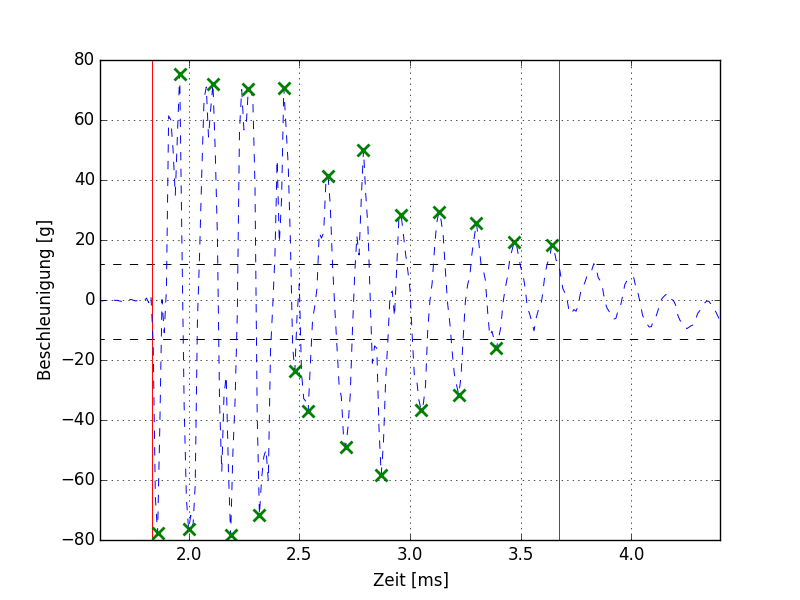
\includegraphics[width=0.95\textwidth]{images/peaks.png}
	\captionof{figure}{Detail-Level 'peaks only'.}
	\label{fig.det_peak}
\end{minipage}%
\begin{minipage}{0.5\textwidth}
\centering
		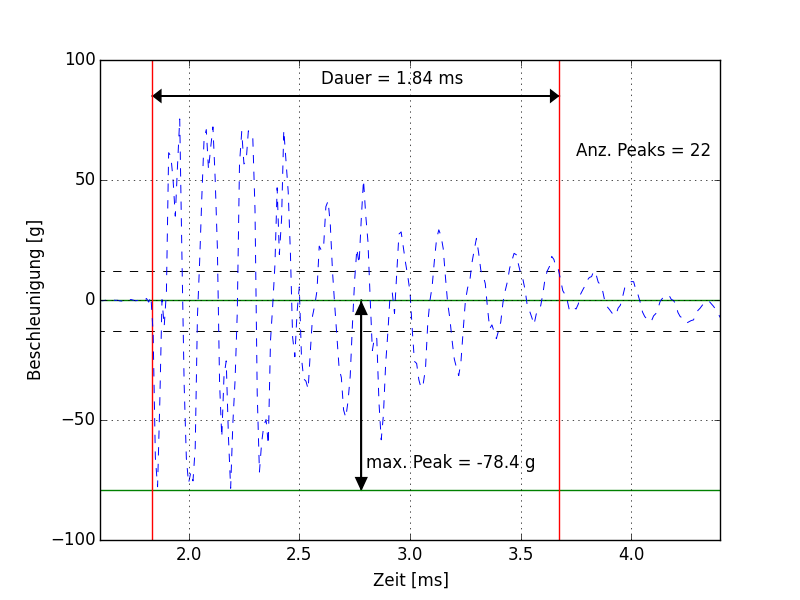
\includegraphics[width=0.95\textwidth]{images/sparse.png}
	\captionof{figure}{Detail-Level 'sparse'.}
	\label{fig.det_sparse}
\end{minipage}
\end{figure}



\subsection{Timestamp}\label{subsec.sw_timestamp}
Der \gls{timestamp} ist ein Zähler, der in jeder \gls{sensoreinh} die gemessenen \glspl{sample} zählt. Die übertragenen \glspl{ereignis} werden mit dem \gls{timestamp} versehen. Der \gls{logger} kann anhand des \gls{timestamp}s, der \gls{fs} der betreffenden \gls{sensoreinh} und des Zeitpunkts des letzten Zurücksetzens der \gls{timestamp}s den Zeitpunkt der Aufnahme des \gls{ereignis}ses berechnen (Gleichung \ref{eq.timestamp}).

\begin{equation}\label{eq.timestamp}
t_{Ereignis} = t_{reset} + (timestamp/fs)
\end{equation}

\section{Busverwaltung}

\subsection{Verwaltung des Bussystems}\label{subsec.sw_busverwaltung}

Da der CAN-Bus für dieses Projekt in einem Internet Protocol (IP) ähnlichen Modus laufen soll, muss der Bus von einer zentralen Stelle verwaltet werden. Ansonsten wäre es schwierig, die einzelnen Teilnehmer am Bus eindeutig zu identifizieren oder zu verhindern, dass ein Sensor auf seinen Daten sitzenbleibt. Abbildungen \ref{fig.seqstartuplogger} und \ref{fig.seqstartupsensor} zeigen die Sequenzen der Verwaltung des Bussystems.
Um das zu garantieren, wird der Datenlogger als Busmaster eingesetzt, der den Sensoren aufgrund einer Konfigurationsdatei und der Mikrocontroller-Seriennummer eine eindeutige CAN-ID zuweist. Hat der \gls{logger} die Seriennummer aller \glspl{sensoreinh} erhalten und diese registriert oder ist vorher ein Timeout aufgetreten, werden die CAN-Identifier verschickt. Als nächstes übermittelt der \gls{logger} allen \glspl{sensoreinh} ihre spezifischen Einstellungen (sofern in der Konfigurationsdatei vorhanden) oder die Standardwerte. Die \gls{sensoreinh} erhalten daraufhin den Timesync-Broadcast des \gls{logger}, der eine Zurücksetzung des Timestamps in den \glspl{sensoreinh} veranlasst. Sobald alle Einstellungen gesetzt wurden, aktiviert der Logger standardmässig den Aufnahmemodus der Sensoren und schickt dem ersten registrierten Sensor den Token zu. Dieser Token enthält auch die maximale Anzahl der Meldungen, die der Sensor dem Logger schicken darf. Der Sensor bestätigt den Token und sendet dem Logger die Anzahl der Meldungen, die er übermitteln wird. So weiss der Logger jederzeit, wieviele Meldungen des Sensors noch ausstehend sind und kann genug Speicher reservieren.

\begin{figure}
	\centering
		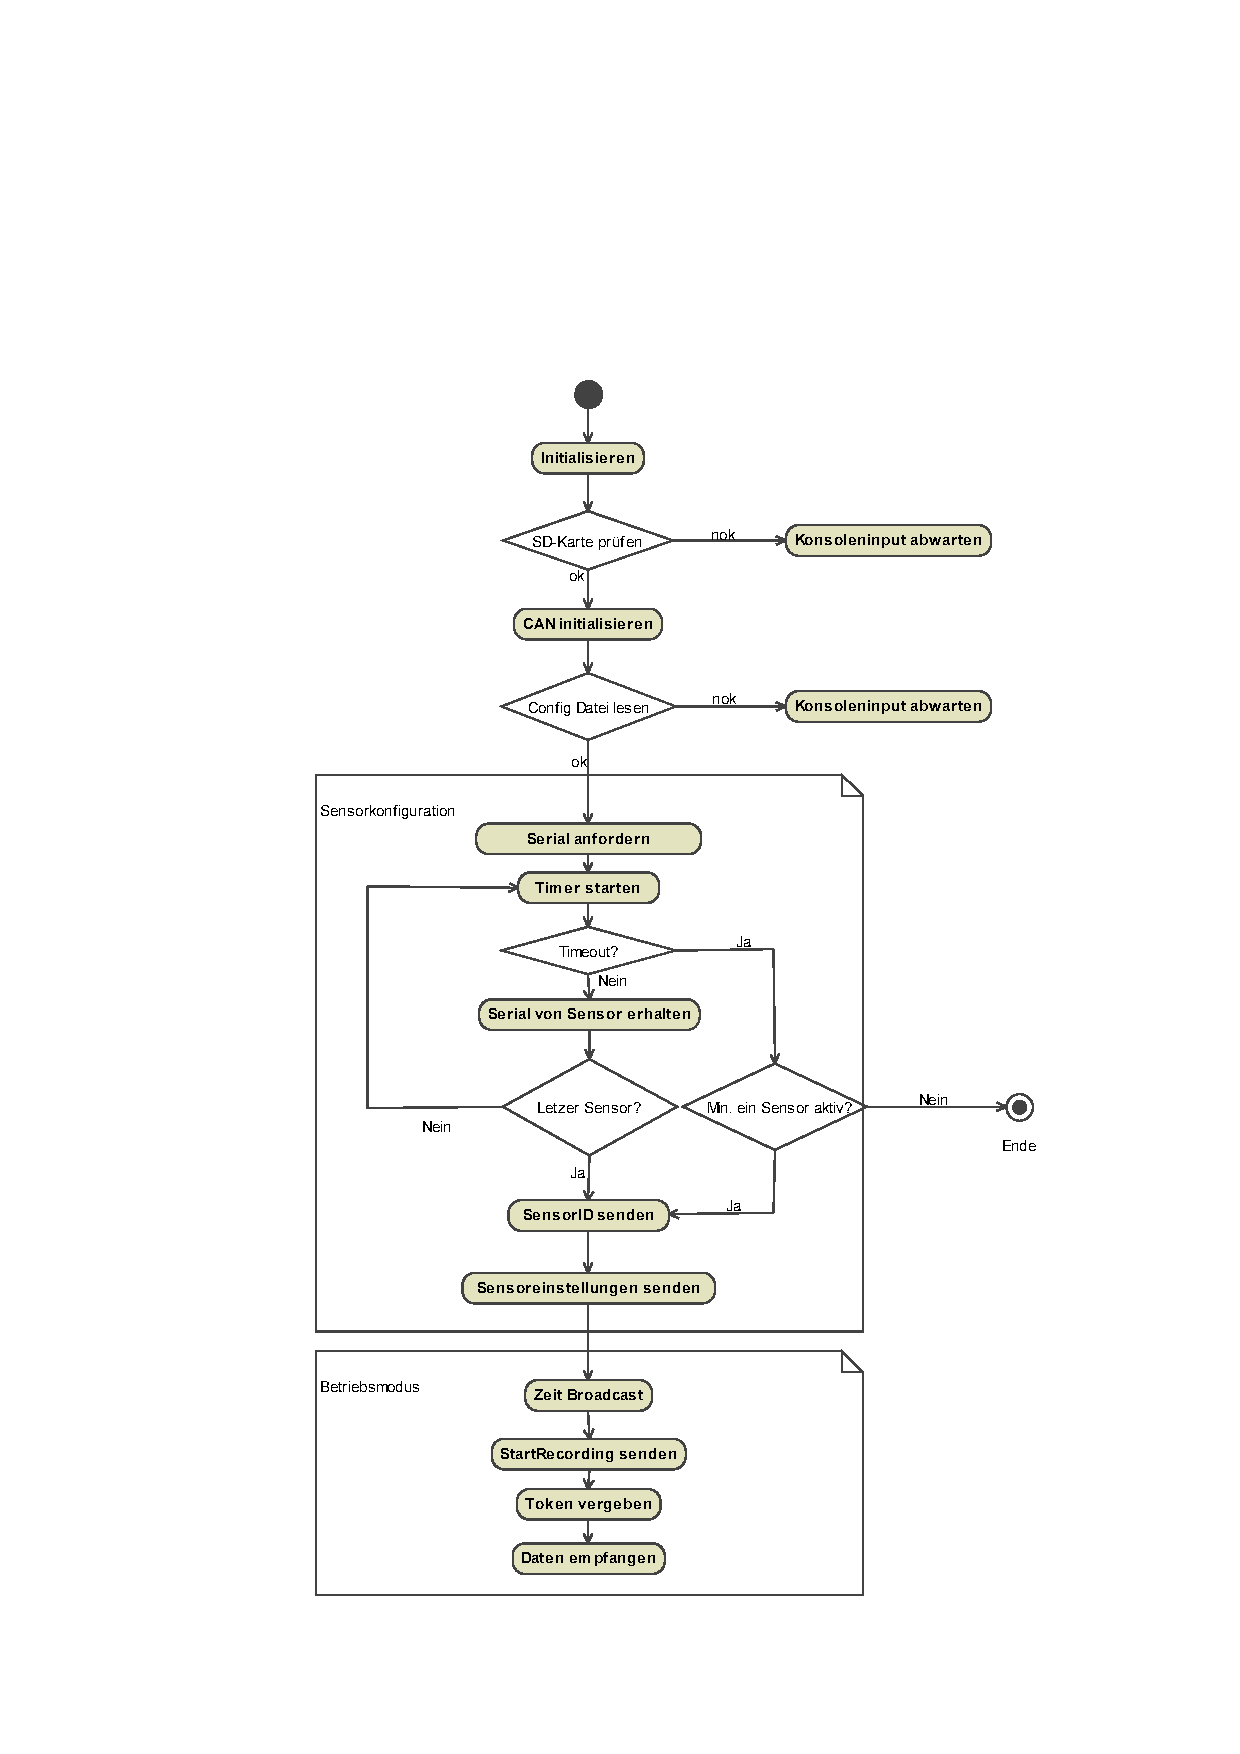
\includegraphics[height=0.9\textheight]{images/magicdraw/AblaufLogger.pdf}
	\caption{Sequenzdiagramm des Startupvorgangs der Messstation.}
	\label{fig.seqstartuplogger}
\end{figure}

Der Start-Ablauf einer \gls{sensoreinh} (Abbildung \ref{fig.seqstartupsensor}) ist das Gegenstück zu dem des \gls{logger}s. Zu Beginn erwartet die \gls{sensoreinh} die Anforderung, ihre Seriennummer bekanntzugeben. Da die \glspl{sensoreinh} keinen persistenten Speicher aufweisen, müssen die Einstellungen jeweils vom  \gls{logger} übermittelt werden. Erhält die \gls{sensoreinh} diese nicht, läuft sie mit den Standardwerten weiter. Beim Eintreffen des Timesync-Broadcasts setzt die \gls{sensoreinh} den Timestamp auf 0 und erwartet den Befehl zum Start der Aufnahme. Sobald dieser eingetroffen ist, wird die Ereigniserkennung gestartet und die \gls{sensoreinh} ist betriebsbereit.

\begin{figure}
	\centering
		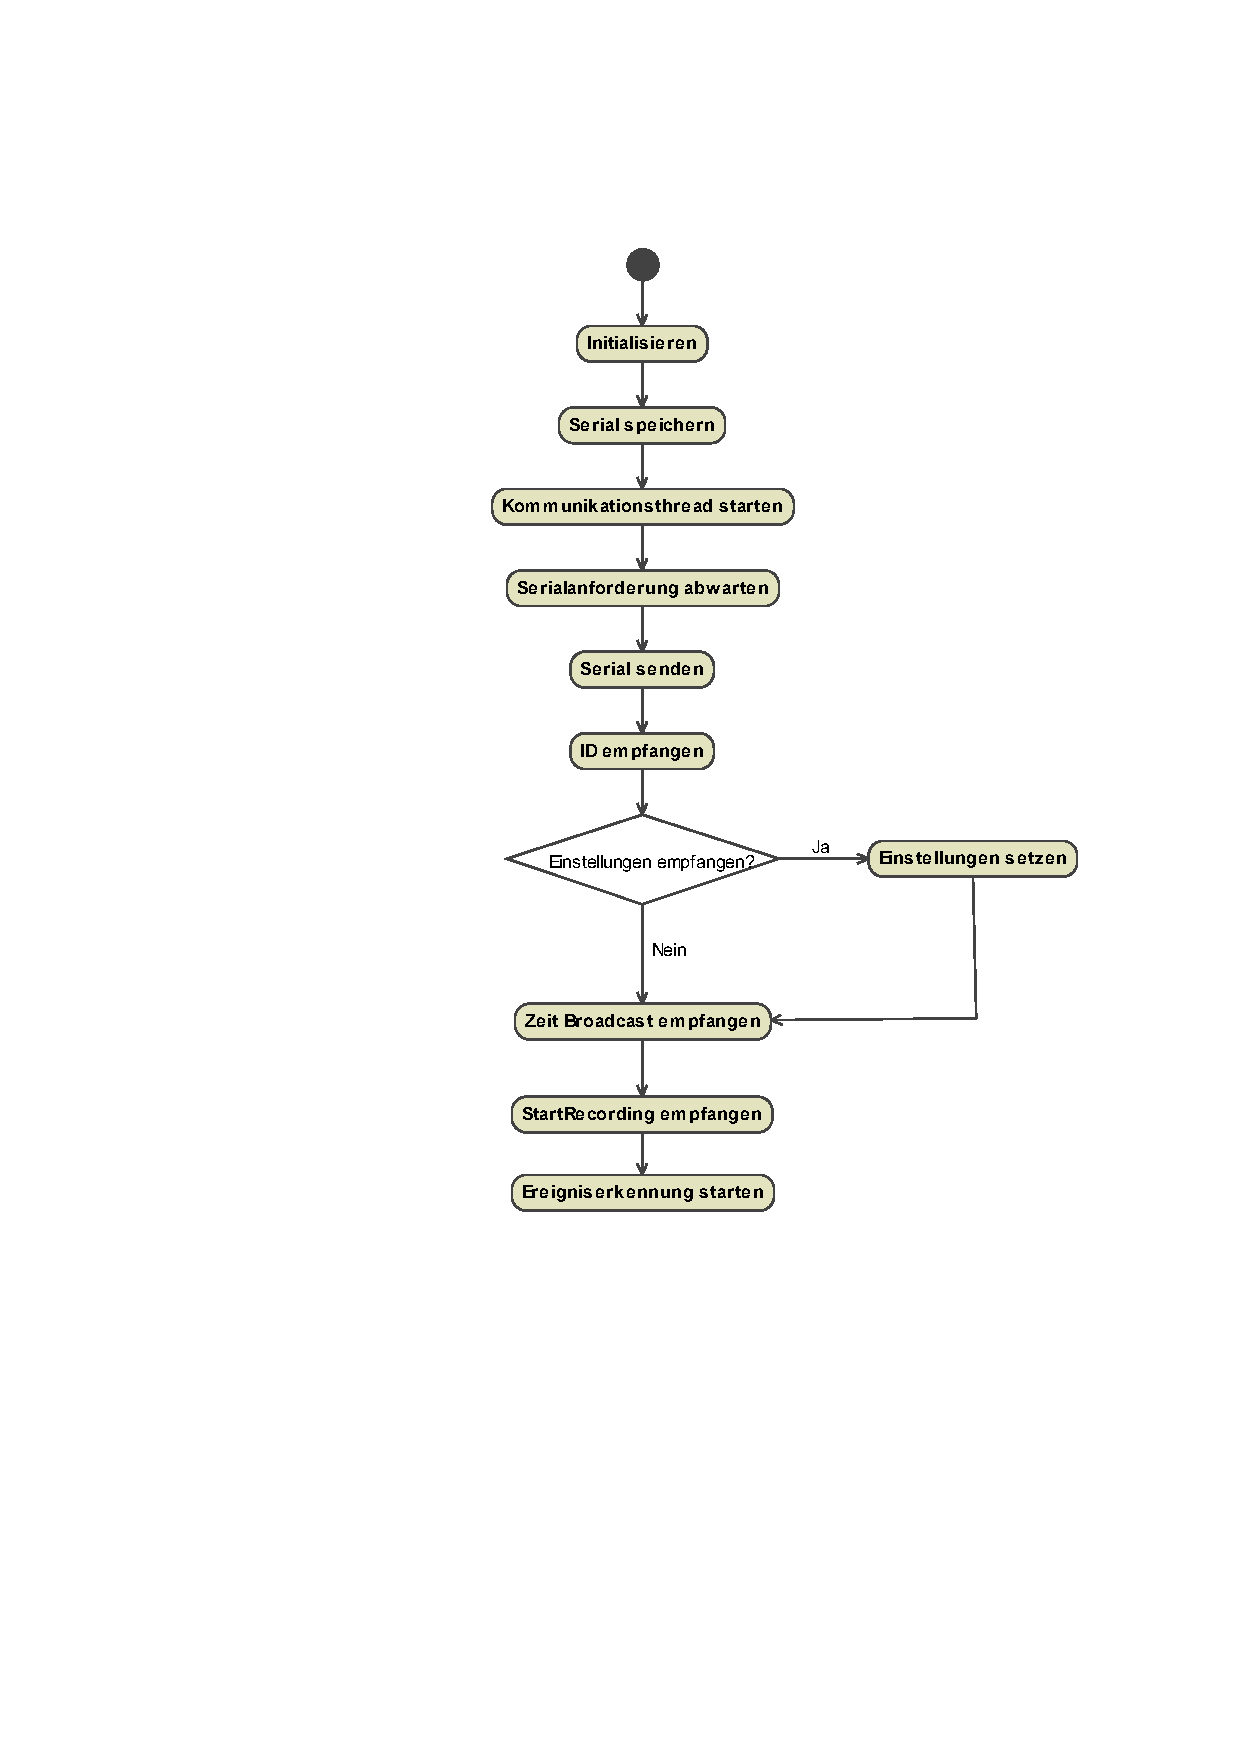
\includegraphics[width=0.8\textwidth]{images/magicdraw/AblaufSensor.pdf}
	\caption{Sequenzdiagramm des Startupvorgangs der Messstation.}
	\label{fig.seqstartupsensor}
\end{figure}


\subsection{Busprotokoll}\label{subsec.sw_busprotokoll}
Ursprünglich wurde das Controller Area Network (CAN) von Bosch entwickelt, um die Steuergeräte in Automobilen zu verbinden \cite{boschcanspec2}. In einem solchen Umfeld ist es wichtig, dass die Kommunikation fehlerfrei und zeitnah erfolgt, da fehlerhafte oder verpasste Meldungen verheerende Folgen nach sich ziehen können (z.B. verpasstes Auslösen des ABS oder der Airbags). Um diese Anforderungen zu erfüllen, wurden einige Vorkehrungen getroffen. Zum einen werden die Daten auf dem CAN-Bus als differenzielles Signal übertragen. Äussere Einflüsse wirken auf beide Leitungen etwa gleich stark und verändern die Differenz deshalb praktisch nicht (siehe auch Abbildung \ref{fig.diff}, Seite \pageref{fig.diff}).

Ein weiteres Problem, dass bei einem Bussystem auftreten kann, sind Daten-Kollisionen zwischen den einzelnen Teilnehmern. Um diese zu verhindern, wird beim CAN das 'Carrier Sense Multiple Access/Collision Resolution'-Verfahren angewandt, bei dem die Teilnehmer zum Sendezeitpunkt feststellen, dass ihre Nachricht mit der eines anderen Teilnehmers kollidiert und dann den Konflikt lösen. Derjenige Sender mit der niedrigeren CAN-ID hat Priorität vor dem anderen Sender, er darf seine Nachricht zu Ende senden \cite{boschcanspec2}. Abbildung \ref{fig.canframe} zeigt den Aufbau eines CAN-Frames im Detail.

Um eine Kollision zu erkennen, prüft jeder Teilnehmer simultan zum Senden, was für ein Signal gerade auf dem Bus anliegt. Stimmt das Bit auf dem Bus mit dem gerade übermittelten überein, ist keine Kollision aufgetreten oder es wurde von allen Teilnehmern gerade ein dominantes Bit (0) übermittelt. Sendet der Teilnehmer im Arbitration-Feld (das aus der Message-ID und einem Control-Bit besteht) ein rezessives Bit und liegt auf dem Bus ein dominantes Bit an, stellt der Teilnehmer seine Übermittlung ein und schickt die Meldung später selbständig erneut \cite{boschcanspec2}. Abbildung \ref{fig.canarbitration} zeigt den Ablauf einer Kollision und ihrer Auflösung mit drei Sendern, die gleichzeitig eine Übertragung starten. 

\begin{figure}
	\centering
		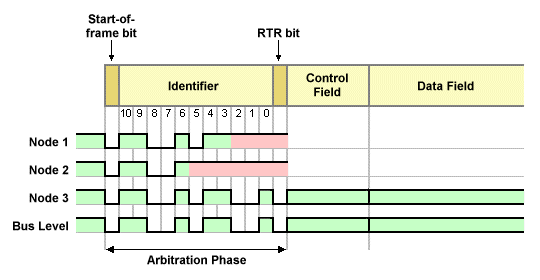
\includegraphics[width=0.8\textwidth]{images/canarbitration.png}
	\caption{Auflösung einer Kollision bei CAN-Bus \cite{canarbit}.}
	\label{fig.canarbitration}
\end{figure}


\begin{figure}
	\centering
		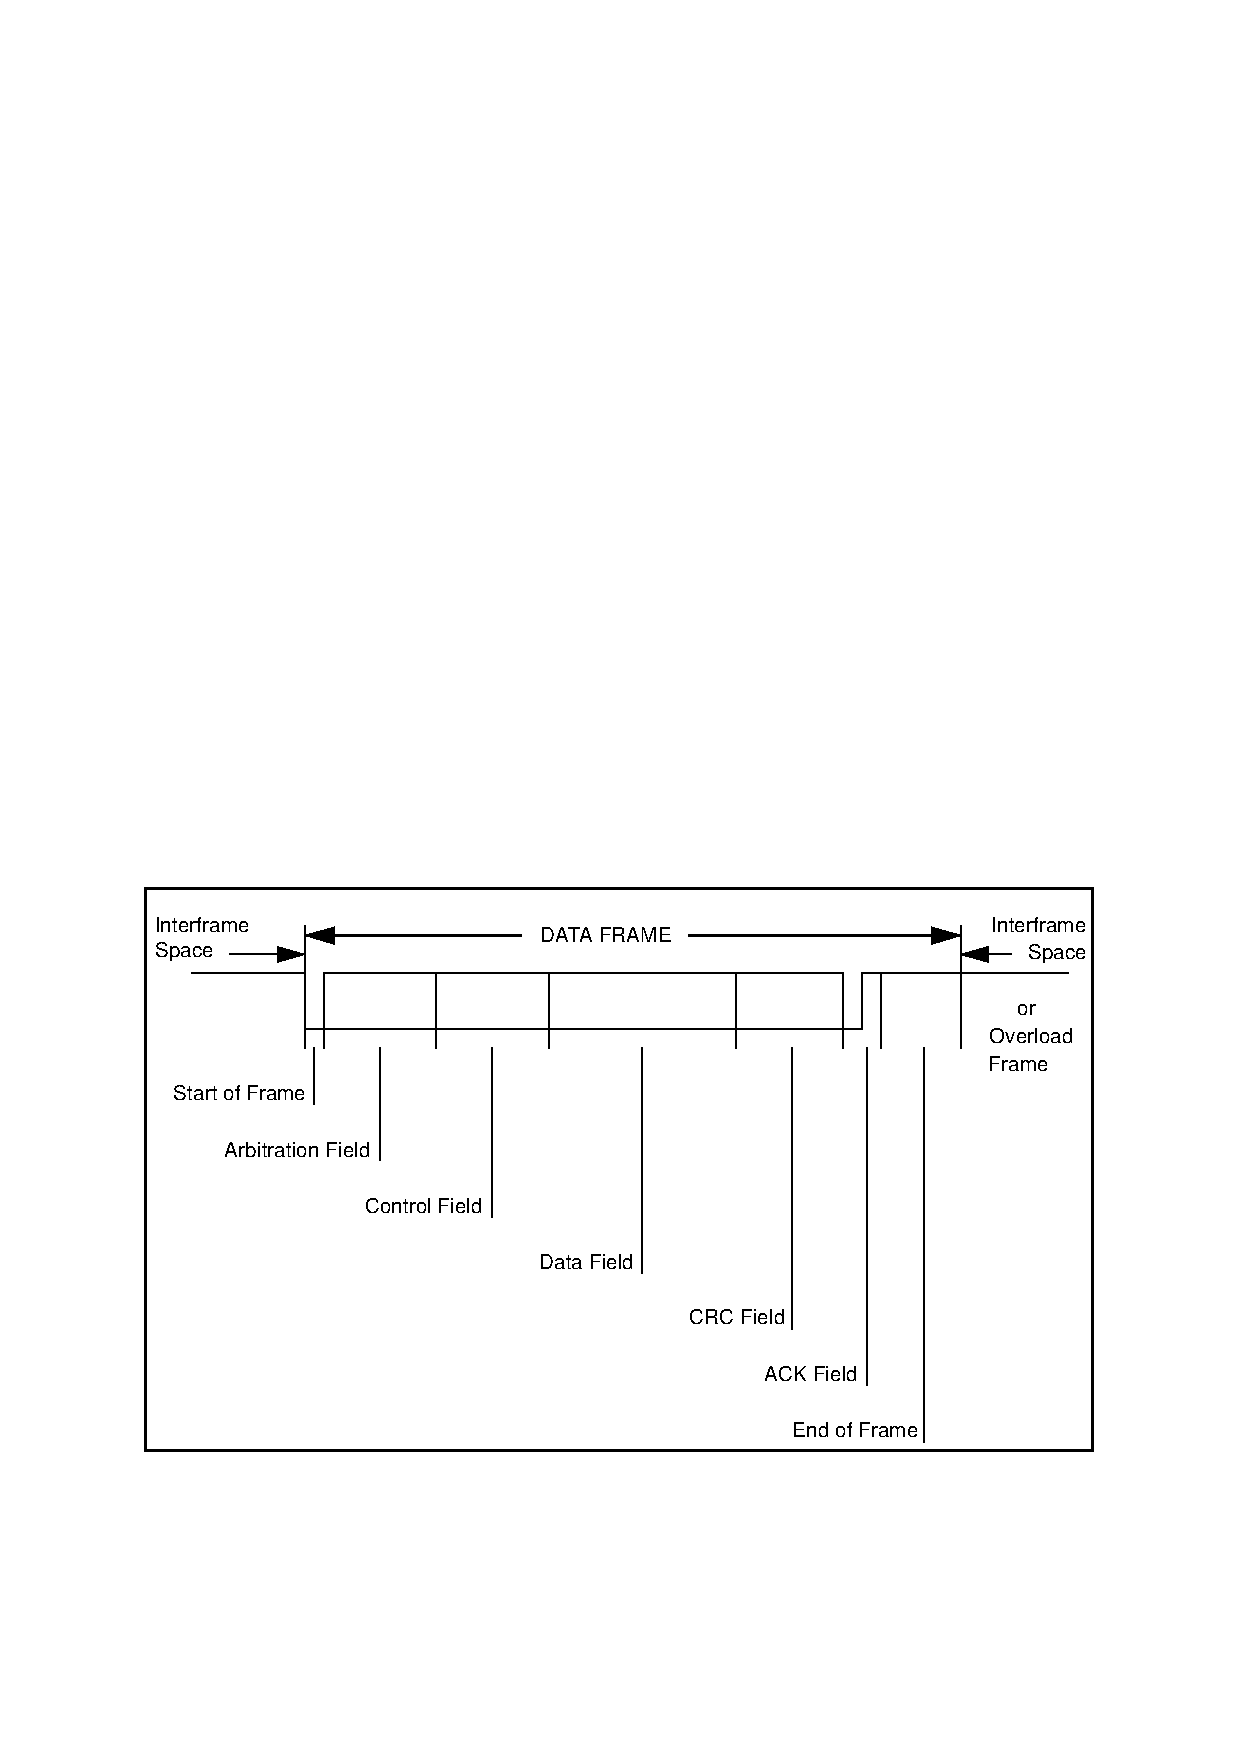
\includegraphics[width=0.8\textwidth]{images/canframe.pdf}
	\caption{Aufbau eines CAN-Frames \cite{boschcanspec2}.}
	\label{fig.canframe}
\end{figure}

\subsubsection{Implementation}
In einem CAN-Bus wird normalerweise kein Bus-Master verwendet, da die Nachrichten nach Verwendungszweck mit IDs versehen sind und so jeder Teilnehmer herausfinden kann, welche Meldungen für ihn relevant sind (zum Beispiel interessiert sich der Auslöser des Airbags nicht für die Abgaswerte der Lambdasonde). Für dieses Bussystem ist aber neben der Art der Meldung auch noch der Absender und der Empfänger wichtig, um einerseits die direkte Kommunikation zwischen dem Datenlogger und einem Sensor und andererseits die Steuerung des Busses per Broadcast-Meldungen zu ermöglichen.



\begin{figure}
	\centering
		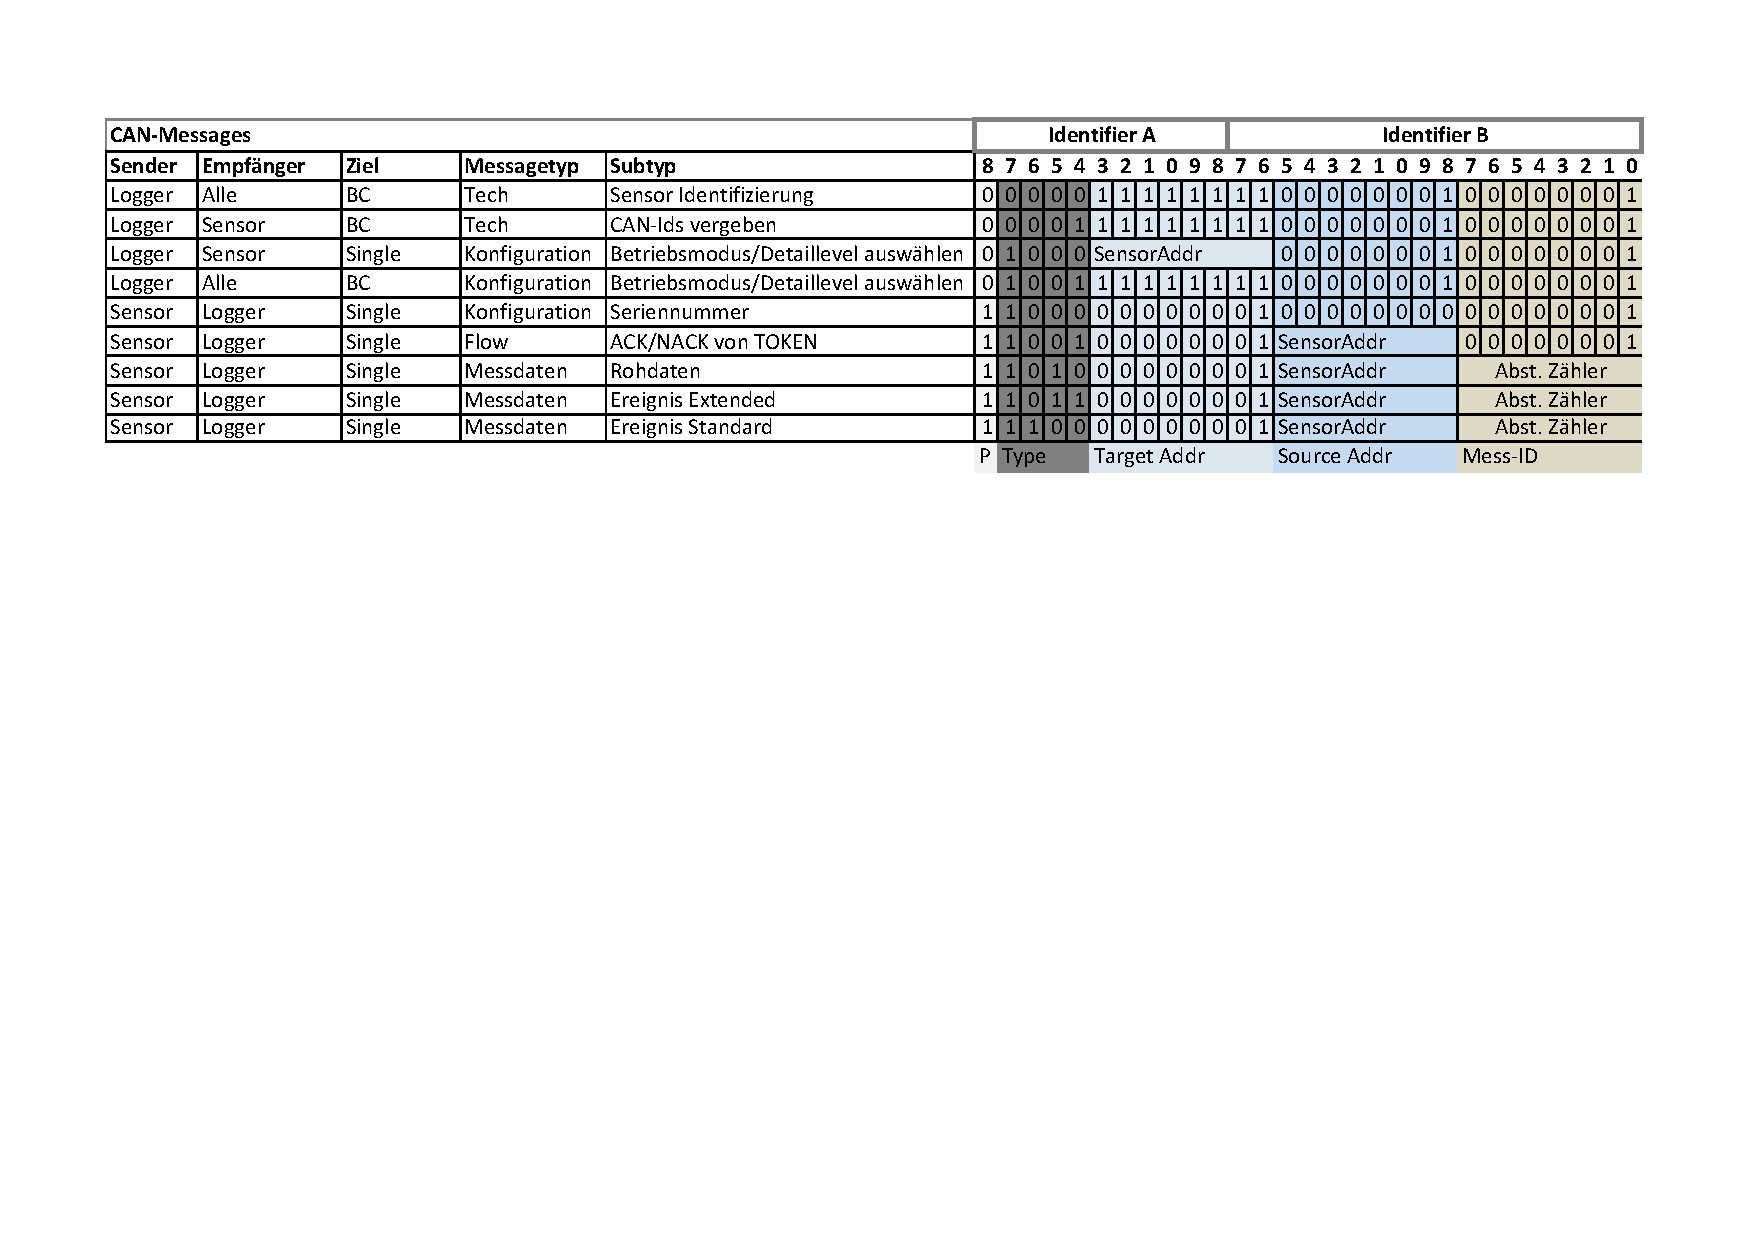
\includegraphics[width=0.8\textwidth]{images/canmess.pdf}
	\caption{Header verschiedener Message-Typen.}
	\label{fig.canmess}
\end{figure}

Da für den Datenlogger wichtig ist, wer welche Daten geschickt hat und die einzelnen Sensoren auch unabhängig voneinander konfiguriert werden müssen, muss jeder Sensor eine eindeutige ID erhalten. Zusätzlich soll unterschieden werden, welcher Art die Nachrichten sind und welche Nachrichten Vorrang haben, falls bei der Übertragung eine Kollision auftritt. Wenn die vorhandenen 11 Bit der Message-ID für den Message-Typ, die Sender- und die Receiveradresse verwendet würden, könnten die Adressen etwa vier Bit ausmachen, es wären also 16 Teilnehmer auf dem Bus erlaubt. Um diese Beschränkung zu umgehen, können Meldungen im „extended format“ geschickt werden. In diesem Format werden Identifier mit einer Länge von 29 Bit zugelassen, welche ausreichen, um den Bus für insgesamt 255 Teilnehmer mit 32 Nachrichtentypen und einem 8 Bit Paketzähler zu  betreiben. Abbildung \ref{fig.canmess} zeigt einige Beispiele der Header von CAN-Frames. Das Busprotokoll mit dem Aufbau aller Nachrichtentypen befindet sich als Excel-Datei auf der beiliegenden CD.

Um sicherzustellen, dass der Busmaster (in diesem Fall der \gls{logger}) immer Priorität vor den anderen Teilnehmern hat, wurde das erste Bit der Message-ID als Prioritätsbit verwendet und für alle Nachrichten vom \gls{logger} auf 0 gesetzt. In der Konfiguration dieses Busses steht eine 0 für ein dominantes Bit, d.h. eine gleichzeitig gesendete 1 würde überschrieben und der andere Teilnehmer erkennt eine Kollision, woraufhin er die Übertragung abbricht und später erneut versucht. Die folgenden vier Bits dienen als Message-Typ (nicht zu verwechseln mit dem CAN-Message Typ, der nicht in der Message-ID vorkommt), welcher an erster Stelle ebenfalls das Prioritätsbit aufweist. Sollten mehr als die bereits verwendeten Message-Typen notwendig werden, kann der volle Bereich ausgeschöpft werden. Die nächsten acht Bits enthalten die Empfängeradresse, darauf folgen die Senderadresse und die eigentliche Message-ID (der Paketzähler). Für eine Broadcast-Message wird die Zieladresse auf 0xFF gesetzt, ansonsten muss der gewünschte Empfänger angegeben werden (0x01 für den Busmaster und eine aufsteigende Nummerierung für jeden Teilnehmer). Als Senderadresse verwenden die noch nicht registrierten Teilnehmer eine leere Sourceadresse, die sonst die zugewiesene CAN-ID des Teilnehmers enthalten sollte. Die Reihenfolge dieser Felder wurde so gewählt, um die Möglichkeit des CAN-Acceptancefilters auszunutzen.

\subsubsection{Acceptance-Filter}
Da nicht jeder am Bus angehängte Teilnehmer alle Nachrichten empfangen muss (eine \gls{sensoreinh} interessiert sich nicht für die Daten einer anderen \gls{sensoreinh} oder die Konfigurationsmeldungen für diese), müssen die irrelevanten Nachrichten ignoriert werden. Dazu gibt es zwei mögliche Ansätze, entweder das Filtern per Software oder die Verwendung des CAN-Acceptance-Filters. Die Filterung per Software kostet zusätzliche Rechenleistung, sollte also nur angewendet werden, wenn die Performance nicht so wichtig ist oder kein Hardwarefilter verfügbar ist.

\begin{figure}
	\centering
		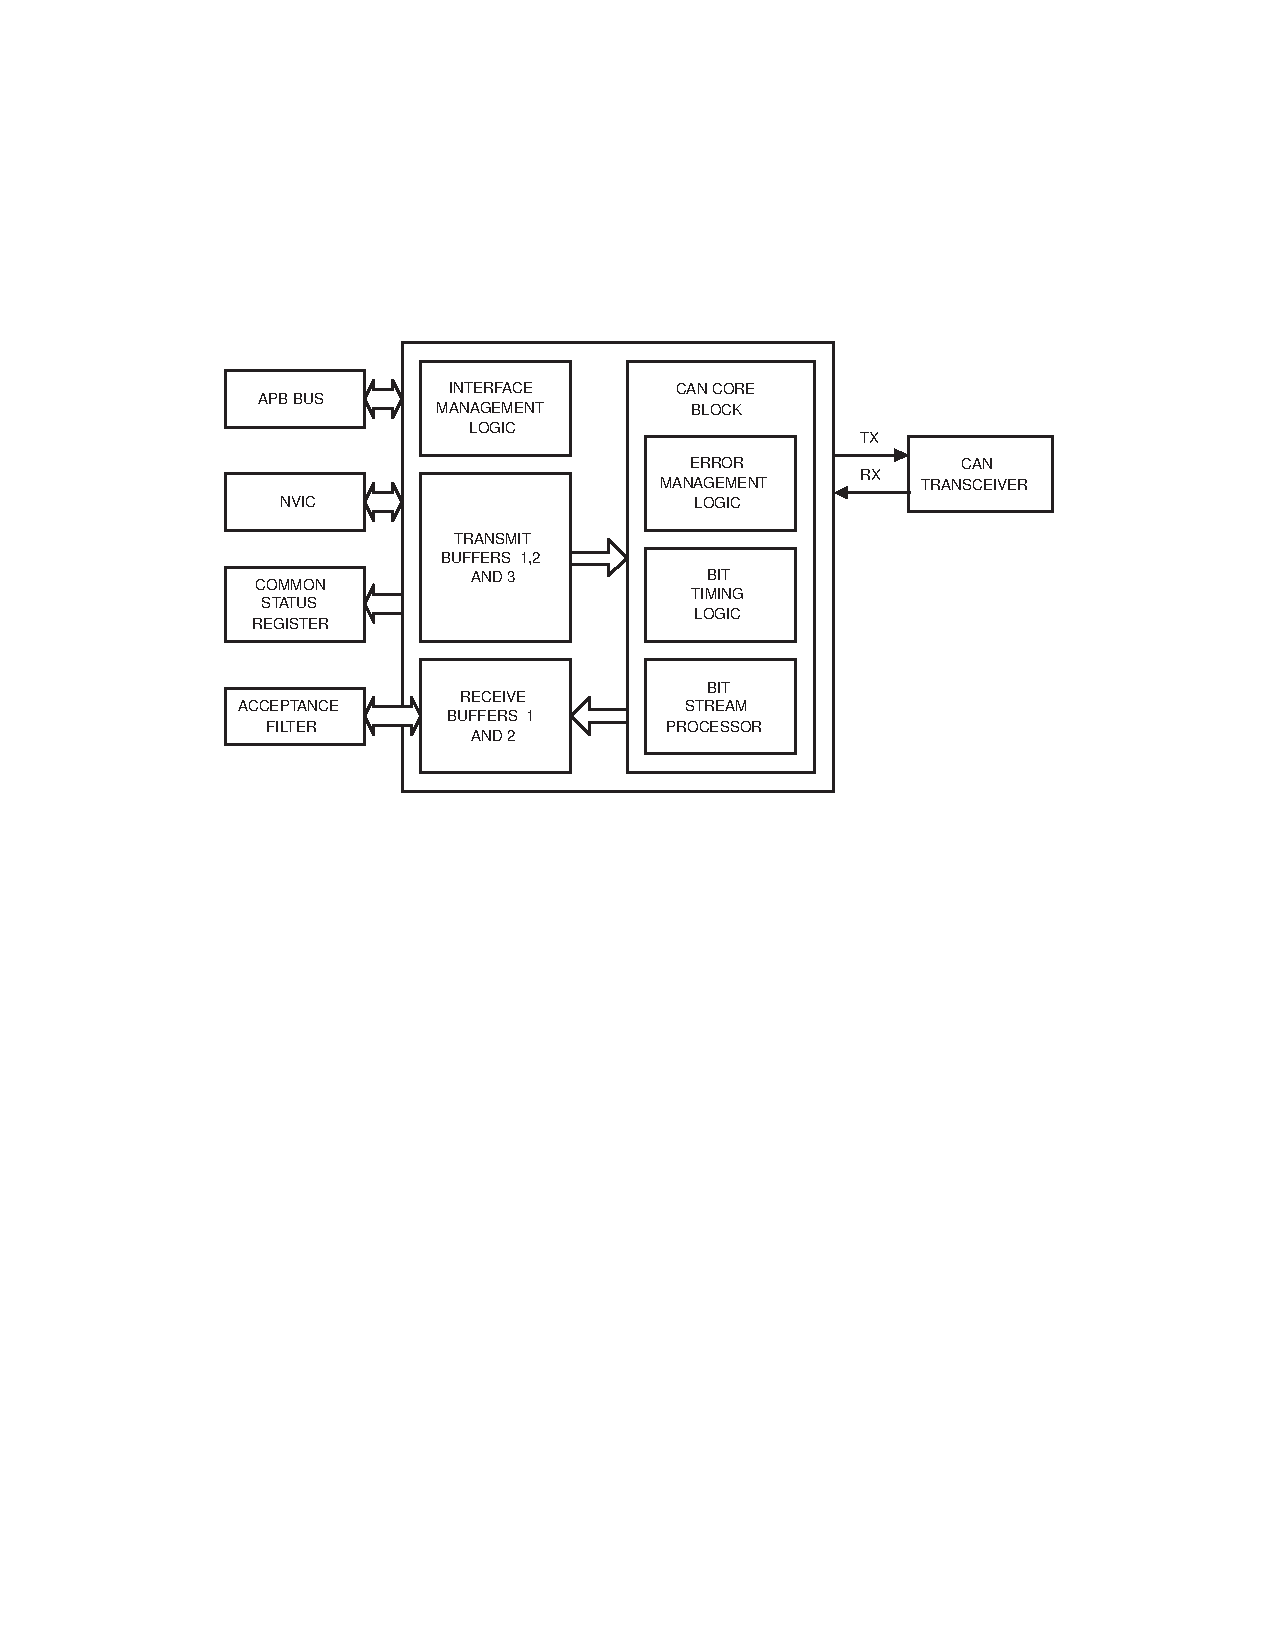
\includegraphics[width=0.8\textwidth]{images/cancontroller.pdf}
	\caption{Schema des CAN-Controllers des NXP LPC4088 \cite{nxplpc4088manual}.}
	\label{fig.cancontroller}
\end{figure}

Im LPC4088 ist für beide CAN-Controller (Abbildung \ref{fig.cancontroller}) ein Hardwarefilter eingebaut, der insgesamt 1024 Standard-Identifier oder 512 Extended Identifier aufnehmen kann. Neben dem spezifischen Filtern, das nur eindeutige Treffer zulässt, kann der Filter auch so konfiguriert werden, dass ganze Bereiche von Message-IDs akzeptiert werden. Zusätzlich besteht noch die Möglichkeit, den Filter in den Full-CAN-Modus zu stellen, bei dem die empfangenen Nachrichten gleich in einem definierten Buffer zwischengespeichert werden, das Auslesen des Empfangsbuffers entfällt hier also. Da dieser Modus aber nur mit spezifischen Standard-Filtern funktioniert, wurde er hier nicht implementiert.

\begin{figure}
	\centering
		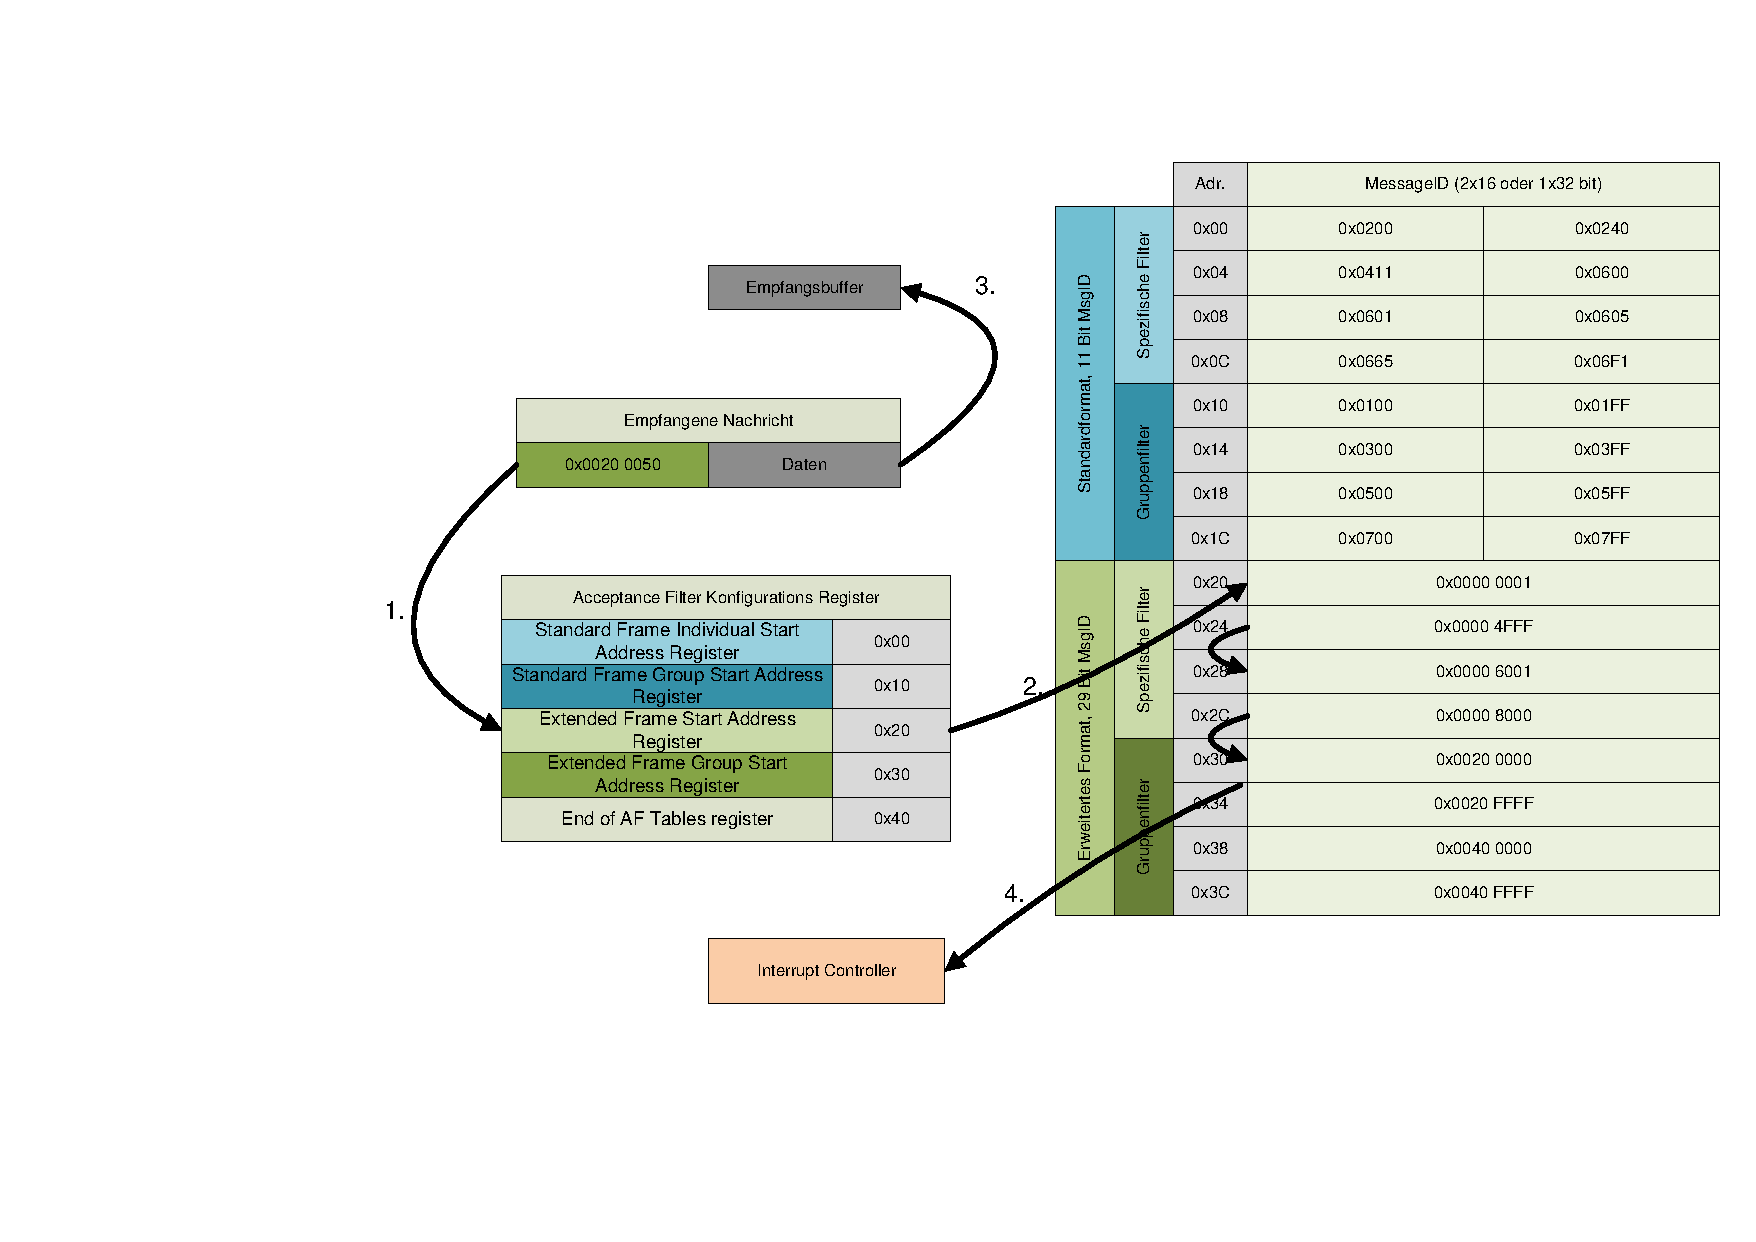
\includegraphics[width=0.9\textwidth]{images/canfilterhit.pdf}
	\caption{Ablauf im CAN-Filter bei Treffer.}
	\label{fig.canfilterhit}
\end{figure}

\begin{figure}
	\centering
		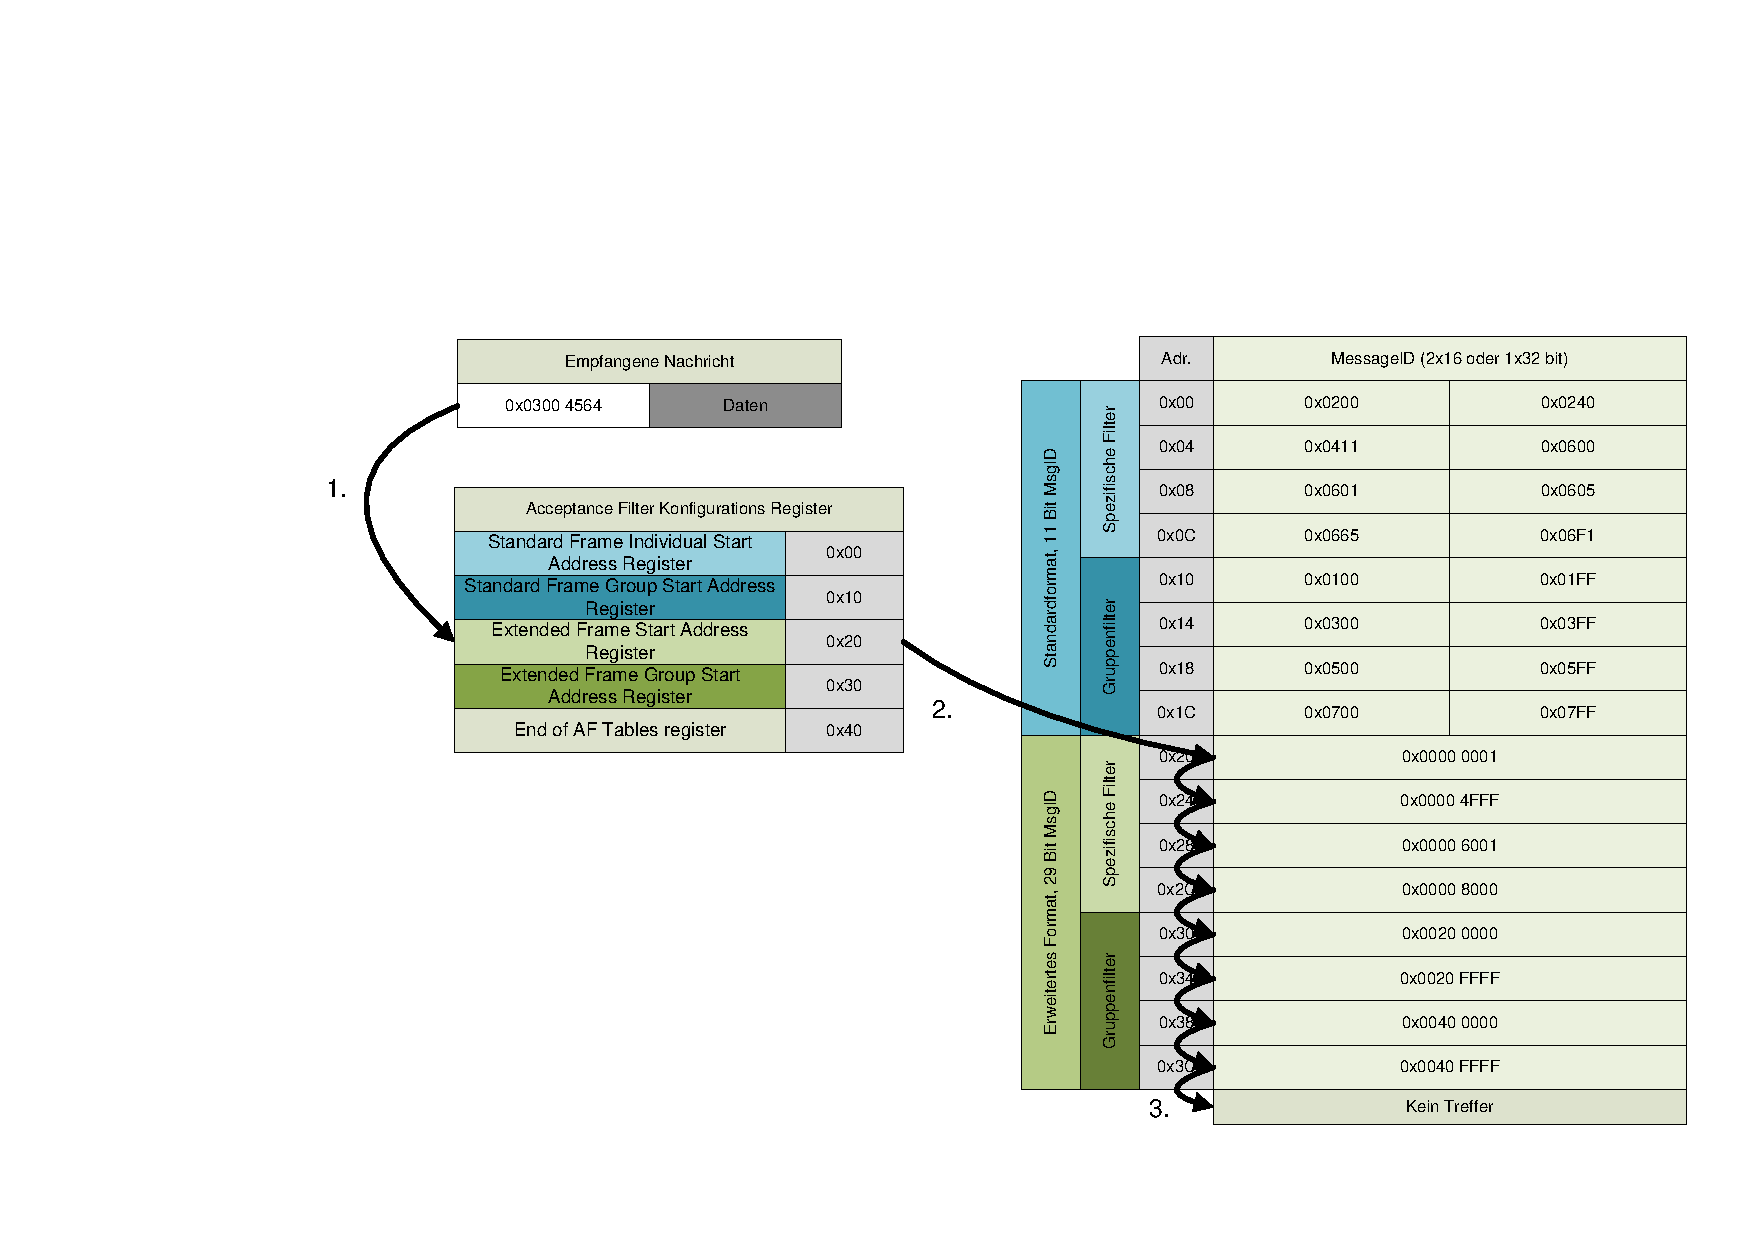
\includegraphics[width=0.9\textwidth]{images/canfiltermiss.pdf}
	\caption{Ablauf im CAN-Filter bei Treffer.}
	\label{fig.canfiltermiss}
\end{figure}

Der Filter (Abbildungen \ref{fig.canfilterhit} und \ref{fig.canfiltermiss}) besteht aus einer Lookup-Tabelle, die hierarchisch aufgebaut ist: zuerst sind die spezifischen Standard-Filter (16 Bit), dann die Gruppen Standard-Filter (2x16 Bit mit lower- und upper-Bound), dann die spezifischen Extended-Filter (32 Bit) und zuletzt die Gruppen Extended-Filter (2x32 Bit) eingetragen. Trifft nun eine CAN-Nachricht ein, wird geprüft, welcher Art die erhaltene Message-ID ist. Im Anschluss wird die ID zuerst gegen die spezifischen Filter geprüft, wird kein Treffer erzielt, werden die Gruppen-Filter geprüft. Bei einem Treffer wird die Nachricht in den Receive-Buffer geladen, der CAN-Controller löst einen Interrupt aus und die ganze Meldung kann ausgelesen werden. Dieser Ablauf mit einem Treffer ist in Abbildung \ref{fig.canfilterhit} dargestellt. Abbildung \ref{fig.canfiltermiss} zeigt den Ablauf, wenn kein Filter zutrifft und die Nachricht ignoriert wird.

Im vorliegenden Bussystem wurden die Filter des Loggers so konfiguriert, dass alle Sensor-Nachrichten akzeptiert werden. Bei den Sensoren wird die Konfiguration des Filters in drei Schritten vorgenommen: nach dem Reset eines Sensors wird der Filter so gesetzt, dass nur eine Seriennummer-Anfrage des Loggers durchgelassen wird. Auf diese Anfrage antworten die Sensoren mit dem versenden ihrer Seriennummer und dem Setzen der Broadcast-Filter. Nun können die Sensoren alle Broadcast-Meldungen des Loggers empfangen. Der Logger verschickt nun die zugeteilten CAN-Ids zusammen mit den entsprechenden Seriennummern als Broadcast. Empfängt ein Sensor den Broadcast, prüft er die Seriennummer und, falls diese mit seiner übereinstimmt, setzt die Filter für alle an ihn gerichteten Meldungen.

\subsection{Filesystem}\label{subsec.sw_filesystem}
Der \gls{logger} legt die Messdaten für jede \gls{sensoreinh} in eine eigene Datei ab. Die Filepointer werden zusammen mit den Konfigurationsdaten im Arbeitsspeicher gehalten. Beim Stoppen einer \gls{sensoreinh} wird die Datei geschlossen und beim erneuten Start der \gls{sensoreinh} eine neue Datei eröffnet. Beim Stopp/Start des \gls{logger}s erfolgt dies für alle Dateien.

Vor dem Entfernen der SD-Karte muss deshalb der \gls{logger} gestoppt werden. Zu diesem Zweck gibt es im Konfigurationsmenü einen eigenen Befehl 'unmount SD card'.

Die Dateinamen haben die Form 'sxx\_MMDD\_hhmm.dat', wobei 'xx' der CAN-ID entspricht, 'MMDD' dem Monat/Tag und 'hhmm' der Stunde/Minute des Starts.

Bei Konfigurationsänderungen schreibt der \gls{logger} einen entsprechenden Eintrag in die Sensordatei. Der Eintrag wird auf eine neue Zeile geschrieben und mit dem Symbol '\#' als Log-Eintrag markiert. Der Eintrag enthält die Uhrzeit und den neuen Wert des Parameters. Am '\#'-Symbol erkennt ein Auswertungsprogramm eine solche Informationszeile und kann diese ignorieren oder bei Bedarf auch entsprechend verarbeiten.



\section{Konfiguration}\label{sec.sw_konfiguration}
Die Konfiguration der Messstation erfolgt einerseits über die Datei 'config.txt', die sich auf der SD-Karte befindet. Andererseits steht über einen \gls{usb}-Anschluss eine serielle Schnittstelle zur Verfügung. Mit einem \gls{terminalemu} kann auf ein Konfigurationsmenü zugegriffen werden, um die Funktionen der Messstation zu steuern.

Die Verwendung der seriellen Schnittstelle über \gls{usb} ist in Abschnitt \ref{ssec.manualserial} der Bedienungsanleitung (ab Seite \pageref{ssec.manualserial}) beschrieben.

Die komplette Beschreibung des Konfigurationsmenüs befindet sich in der Bedienungsanleitung ab Abschnitt \ref{ssec.menu}, Seite \pageref{ssec.menu}.
